% !TEX program = xelatex
% !TEX TS-program = xelatex
\documentclass[a4paper,12pt]{report}
\usepackage[margin=0.85in]{geometry}
\usepackage{graphicx}
\usepackage{parskip}
\usepackage{listings}
\usepackage{titlesec}
\usepackage{setspace}
\usepackage{float}
\usepackage{xcolor}
\usepackage{amssymb}
\usepackage{etoolbox}
\usepackage{fancyhdr}
\usepackage{iftex}

% ---------- FONT SPECIFICATION: TIMES NEW ROMAN EVERYWHERE ----------
\ifxetex
  \usepackage{fontspec}
  \setmainfont{Times New Roman}
  \setsansfont{Times New Roman}
  \setmonofont{Times New Roman}
\else\ifluatex
  \usepackage{fontspec}
  \setmainfont{Times New Roman}
  \setsansfont{Times New Roman}
  \setmonofont{Times New Roman}
\else
  % pdfLaTeX fallback: Times font with all families mapped to roman
  \usepackage[utf8]{inputenc}
  \usepackage[T1]{fontenc}
  \usepackage{mathptmx}
  \renewcommand{\familydefault}{\rmdefault}
  \renewcommand{\sfdefault}{\rmdefault}
  \renewcommand{\ttdefault}{\rmdefault}
\fi\fi

\setlength{\parindent}{1cm}
\setlength{\parskip}{6pt}
\setstretch{1.5}
\setcounter{tocdepth}{3}
\setcounter{secnumdepth}{3}
\frenchspacing

% ---------- Student details ----------
\newcommand{\studentname}{SAMEER SHA}
\newcommand{\rollno}{CHN25MCA-2045}
\newcommand{\guidename}{Smt. Beena K}

% ---------- Colours and code style ----------
\definecolor{codegreen}{rgb}{0,0.6,0}
\definecolor{codegray}{rgb}{0.5,0.5,0.5}
\definecolor{codepurple}{rgb}{0.58,0,0.82}

\lstdefinestyle{customcsharp}{
	language=[Sharp]C,
	basicstyle=\small\rmfamily,
	keywordstyle=\color{blue},
	commentstyle=\color{codegreen},
	stringstyle=\color{orange},
	showstringspaces=false,
	breaklines=true,
	frame=single,
	numbers=left,
	numberstyle=\tiny\color{codegray},
	numbersep=5pt,
	tabsize=2,
	captionpos=b
}

% ---------- Headings (All rmfamily - Times New Roman) ----------
\renewcommand{\chaptername}{CHAPTER}
\let\mtcontentsname\contentsname
\renewcommand\contentsname{\MakeUppercase\mtcontentsname}
\renewcommand{\listfigurename}{LIST OF FIGURES}
\renewcommand{\listtablename}{LIST OF TABLES}

\titleformat{\chapter}[display]
{\normalfont\rmfamily\Large\bfseries\centering}
{\chaptertitlename\ \thechapter}{0pt}{\Large}

\titlespacing*{\chapter}{0pt}{0pt}{6pt}
\titlespacing*{\section}{0pt}{0pt}{6pt}
\titlespacing*{\subsection}{0pt}{0pt}{6pt}
\titlespacing*{\subsubsection}{0pt}{0pt}{6pt}

\titleformat*{\section}{\normalfont\rmfamily\Large\bfseries}
\titleformat*{\subsection}{\normalfont\rmfamily\large\bfseries}
\titleformat*{\paragraph}{\normalfont\large\rmfamily}
\titleformat*{\subsubsection}{\normalfont\rmfamily\large\itshape}

% ---------- Stop \cite from printing inside the lists of figures/tables ----------
\makeatletter
\let\oldcite\cite
\pretocmd{\listoffigures}{\def\cite{\ignorespaces\@gobble}}{}{}
\apptocmd{\listoffigures}{\let\cite\oldcite}{}{}
\pretocmd{\listoftables}{\def\cite{\ignorespaces\@gobble}}{}{}
\apptocmd{\listoftables}{\let\cite\oldcite}{}{}
\makeatother

\begin{document}
	
	% =====================================================================
	%  COVER PAGE
	% =====================================================================
	\begin{minipage}{0.9\linewidth}
		\centering
		
		\vspace{1.5cm}
		\Large\textbf{\uppercase{NETSENTINEL}}\\
		\vspace{0.3cm}
		\large\textbf{Network Traffic Analyzer and Intrusion Detection System}\\
		\normalsize\textbf{A Web-Based Platform for Real-Time Network Monitoring and Threat Detection}\\
		\vspace{0.8cm}
		
		{\uppercase{\large{{MINI PROJECT REPORT}\par}}}
		\vspace{0.4cm}
		\large{Submitted by}
		
		\vspace{0.4cm}
		{\large \textbf{\studentname \\ \rollno}\par}
		\vspace{0.4cm}
		to
		\vspace{0.4cm}
		
		\textit{APJ Abdul Kalam Technological University \\ in partial fulfillment of the requirements for the award of Degree
			in \textbf{Master of Computer Applications}}
		
		\vspace{1.2cm}
		\IfFileExists{CEC.png}{
\includegraphics[width=0.28\textwidth]{CEC.png}}{}
		\vspace{0.8cm}
		
		\large{\textbf{DEPARTMENT OF COMPUTER ENGINEERING\\
				COLLEGE OF ENGINEERING CHENGANNUR, ALAPPUZHA\\
				OCTOBER 2026\\}}
	\end{minipage}
	\thispagestyle{empty}
	\clearpage
	
	% =====================================================================
	%  CERTIFICATE
	% =====================================================================
	\thispagestyle{empty}
	
	\begin{center}
		\vspace{1.2cm}
		
		\textbf{DEPARTMENT OF COMPUTER ENGINEERING \\}
		\textbf{COLLEGE OF ENGINEERING CHENGANNUR\\}
		\textbf{ALAPPUZHA}
	\end{center}
	
	\begin{center}
		\IfFileExists{CEC.png}{
\includegraphics[width=0.25\textwidth]{CEC.png}}{}
	\end{center}
	
	\begin{center}
		\textbf{CERTIFICATE}
	\end{center}
	
	\begin{spacing}{1.5}
		\textit{This is to certify that the project report titled \textbf{NETSENTINEL: NETWORK TRAFFIC ANALYZER AND INTRUSION DETECTION SYSTEM} is a bonafide record of the \textbf{20MCA245 MINI PROJECT} presented by \textbf{\studentname} (\rollno), Third Semester Master of Computer Applications student, under our guidance and supervision. This project is submitted in partial fulfillment of the requirements for the award of the degree \textbf{Master of Computer Applications} of \textbf{APJ Abdul Kalam Technological University}.}
	\end{spacing}
	
	% Signature block
	\begin{singlespace}
		\vspace*{0.8cm}
		
		\noindent
		\begin{tabular*}{\textwidth}{@{\extracolsep{\fill}} l l}
			\textbf{\guidename} & \textbf{Smt. Josmi Jose} \\
			Project Guide & Project Coordinator \\
			Assistant Professor & Assistant Professor \\
			Dept. of Computer Engineering & Dept. of Computer Engineering \\[1.2cm]
		\end{tabular*}
		
		\begin{center}
			\textbf{Dr. Renu George} \\
			Professor \\
			Head of the Department \\
			Dept. of Computer Engineering
		\end{center}
	\end{singlespace}
	\clearpage
	
	\pagenumbering{roman}
	
	% =====================================================================
	%  DECLARATION
	% =====================================================================
	\addcontentsline{toc}{chapter}{Declaration}
	\begin{center}
		\Large {\bf \uppercase{Declaration}}
	\end{center}
	\vspace{1cm}
	
	\noindent I undersigned hereby declare that the project report \textbf{NETSENTINEL: NETWORK TRAFFIC ANALYZER AND INTRUSION DETECTION SYSTEM}'', submitted for partial fulfillment of the requirements for the award of degree of Master of Computer Application of the APJ Abdul Kalam Technological University, Kerala is a bonafide work done by me under the supervision of \textbf{\guidename}, Assistant Professor, Department of Computer Engineering. This submission represents my ideas in my own words, and where ideas or words of others have been included, I have adequately and accurately cited and referenced the original sources. I also declare that I have adhered to the ethics of academic honesty and integrity and have not misrepresented or fabricated any data, idea, fact, or source in this submission. I understand that any violation of the above will be a cause for disciplinary action by the institute and/or the University and can also evoke penal action from the sources which have thus not been properly cited or from whom proper permission has not been obtained. This report has not been previously formed the basis for the award of any degree, diploma, or similar title of any other University.
	
	\vspace{3.5cm}
	
	\noindent\begin{minipage}{0.45\linewidth}
		\begin{flushleft}
			\textbf{Place:} Chengannur \\
			\textbf{Date :}
		\end{flushleft}
	\end{minipage}
	\hfill
	\begin{minipage}{0.45\linewidth}
		\begin{flushright}
			\textbf{\studentname}\\
			\textbf{\rollno}\\
		\end{flushright}
	\end{minipage}
	\clearpage
	
	% =====================================================================
	%  ACKNOWLEDGEMENT
	% =====================================================================
	\addcontentsline{toc}{chapter}{Acknowledgement}
	\begin{center}
		\Large {\bf \uppercase{Acknowledgement}}
	\end{center}
	\vspace{1.2cm}
	
	\noindent This work would not have been possible without the support, guidance, and cooperation of many individuals. First and foremost, I offer my humble gratitude to Almighty God, whose grace, blessings, and strength enabled me to undertake and successfully complete this project work.
	
	I would like to express my sincere gratitude to \textbf{Dr. Hari V.S}, The Principal, College of Engineering Chengannur, for providing the necessary facilities, infrastructure, and academic atmosphere conducive to project development. I extend my deep appreciation to \textbf{Dr. Renu George}, Professor and Head of the Department of Computer Engineering, for her continuous support, administrative facilitation, and encouragement throughout the semester.
	
	I am profoundly grateful to my project guide, \textbf{\guidename}, Assistant Professor, Department of Computer Engineering, for her invaluable guidance, technical suggestions, constructive critiques, and constant encouragement at every stage of the project. I also extend my sincere thanks to our project coordinators, \textbf{Smt. Josmi Jose}, \textbf{Smt. Santhy Viswam}, and \textbf{Smt. Celin T}, Assistant Professors, Department of Computer Engineering, for their meticulous planning, periodic evaluations, and timely guidance.
	
	Finally, I express my heartfelt gratitude to all faculty members of the Department of Computer Engineering, my dear classmates, and my family members for their unwavering moral support, valuable feedback, and encouragement throughout this endeavour.
	
	\begin{flushright}
		\textbf{\studentname\\\rollno}
	\end{flushright}
	\clearpage
	
	% =====================================================================
	%  ABSTRACT
	% =====================================================================
	\addcontentsline{toc}{chapter}{Abstract}
	\begin{center}
		\Large\textbf{ABSTRACT}
	\end{center}
	\vspace{1cm}
	
	Network security monitoring in contemporary digital environments is frequently impaired by the high volume of raw network telemetry, the operational complexity of legacy packet inspection utilities, and the lack of accessible, unified visualization platforms. Traditional command-line packet sniffers and standalone intrusion detection engines require specialized expertise to configure, lack integrated multi-host tracking, and fail to provide immediate, actionable situational awareness for security analysts. To address these operational challenges, this project presents NetSentinel, a comprehensive web-based Network Traffic Analyzer and Intrusion Detection System engineered to deliver real-time packet inspection, automated behavioral threat detection, and centralized security operations management. NetSentinel incorporates a decoupled, multi-tier architecture comprising a high-performance Python packet capture and intrusion detection engine, a robust Node.js and Express RESTful application programming interface with Socket.io WebSocket event streaming, an enterprise MySQL relational database, and an interactive React web dashboard designed with a soft claymorphic aesthetic. The Python engine captures live Layer 3 and Layer 4 packets using Scapy or generates reproducible multi-host traffic through an integrated synthetic simulator, evaluating telemetry against configurable sliding-window heuristic detection rules for SYN floods, port scans, ICMP floods, suspicious DNS activity, malicious payloads, and malformed headers. Detected anomalies trigger immediate database alerts with a thirty-second cooldown cache and stream instantaneously to connected clients. The platform enforces strict role-based access control between security analysts and administrators, facilitating real-time throughput charting, protocol distribution breakdown, automated host discovery with threat scoring, alert triage, rule tuning, and on-demand generation of executive PDF and raw CSV forensic reports. By integrating wire-speed packet ingestion, explainable signature detection, and responsive telemetry visualization into a cohesive web platform, NetSentinel significantly improves network observability, threat triage efficiency, and security operations management.
	
	\clearpage
	
	% =====================================================================
	%  CONTENTS, LISTS
	% =====================================================================
	\tableofcontents
	\newpage
	
	\addcontentsline{toc}{chapter}{List of Figures}
	\listoffigures
	\newpage
	
	\addcontentsline{toc}{chapter}{List of Tables}
	\listoftables
	\clearpage
	
	% =====================================================================
	%  CHAPTER 1
	% =====================================================================
	\pagenumbering{arabic}
	\chapter{INTRODUCTION}
	
	\section{Project Area}
	\par
	Modern digital communication networks serve as the backbone for organizational operations, enterprise resource access, cloud computing, and industrial automation. As institutions and corporate enterprises connect heterogeneous computing nodes across local area networks and distributed internet gateways, the volume, velocity, and architectural heterogeneity of network packets increase exponentially. Securing these environments requires continuous visibility into communications occurring across Layer 3 (Network) and Layer 4 (Transport) protocols. In the absence of structured, automated surveillance, malicious cyber operations such as distributed denial-of-service volumetric floods, reconnaissance scanning probes, command-and-control communication tunneling, and application-layer exploit attempts can traverse internal network segments without triggering timely defensive responses.
	
	Conventional network security practices frequently depend on decentralized, isolated monitoring utilities. Command-line diagnostic tools such as tcpdump, specialized packet capture utilities like Wireshark, and heavy enterprise Intrusion Detection Systems (IDS) often impose steep operational barriers. Command-line tools require security personnel to manually formulate complex packet capture filters and parse high-density hexadecimal packet dumps, which impedes rapid situational assessment during ongoing cyber incidents. Conversely, enterprise commercial monitoring suites demand significant computational overhead, complex cluster deployments, and proprietary agent installations on every client host. Furthermore, traditional utilities frequently lack integrated web-based dashboards capable of translating raw packet captures into intuitive, real-time graphical representations of throughput, bandwidth utilization, host inventory, and incident severity.
	
	`\textbf{NetSentinel}'' is designed and implemented as a full-stack, real-time Network Traffic Analyzer and Intrusion Detection System that unifies live packet interception, rule-based behavioral threat analysis, relational telemetry persistence, and claymorphic web visualization. Developed with a decoupled architecture, NetSentinel employs a Python-based packet capture service using Scapy alongside an enterprise Node.js Express RESTful backend, a MySQL 8.4 database, and a React web dashboard. The system incorporates dual operational modes—a live interface sniffer for physical and wireless network cards and a synthetic multi-host simulator for controlled security evaluations—while enforcing strict role-based access control between Standard Users (Security Analysts) and Administrators. Designed for rapid deployment in local network environments, NetSentinel provides extensible sliding-window detection rules, automated host discovery with behavioral risk scoring, and one-click PDF and CSV forensic export capabilities.
	
	\section{Objectives}
	\begin{enumerate}
		\item \textbf{To develop a centralized real-time packet capture and ingestion pipeline:}
		The system aims to capture live Ethernet, Wi-Fi, and simulated multi-host IP packets continuously, extracting protocol headers, IP addresses, port numbers, packet lengths, and TCP control flags for real-time security analysis.
		
		\item \textbf{To engineer a multi-rule sliding-window intrusion detection engine:}
		The system aims to implement stateful and heuristic detection algorithms capable of identifying volumetric SYN floods, reconnaissance port scans, ICMP echo floods, suspicious DNS queries, signature-based payload attacks, and malformed network packets.
		
		\item \textbf{To implement automated network device discovery and risk scoring:}
		The system aims to inspect observed traffic dynamically to identify active network hosts, resolve IP and MAC address pairs, classify hardware types, and compute empirical behavioral risk scores based on detected incident history.
		
		\item \textbf{To establish an asynchronous event streaming and telemetry architecture:}
		The system aims to stream live throughput metrics, bandwidth statistics, protocol distributions, and threat alerts from the backend ingestion controllers to connected browser sessions using WebSocket communication.
		
		\item \textbf{To provide strict role-based access control and administrative governance:}
		The system aims to enforce distinct privilege levels between read-only Security Analysts and SecOps Administrators, restricting capture engine execution, rule sensitivity tuning, alert triage, and user management to verified administrative users.
		
		\item \textbf{To deliver an interactive, responsive claymorphic web dashboard:}
		The system aims to present comprehensive network intelligence through responsive Chart.js line and donut visualizations, real-time packet tables, and an interactive threat investigation drawer displaying hexadecimal payload previews.
		
		\item \textbf{To generate standardized executive PDF and raw forensic CSV reports:}
		The system aims to compile structured audit documentation and raw forensic packet archives on demand across configurable historical time windows to support compliance audits and forensic analysis.
		
		\item \textbf{To provide a dual-mode execution environment with synthetic attack simulation:}
		The system aims to support both elevated physical packet sniffing via Npcap and an integrated synthetic multi-host traffic simulator that enables offline security testing, education, and benchmark verification without external hardware dependencies.
	\end{enumerate}
	
	% =====================================================================
	%  CHAPTER 2
	% =====================================================================
	\chapter{LITERATURE REVIEW}
	
	\section{Network Traffic Analyzer: Real-Time Detection and Malicious Activity Identification}
	\par
	This research paper, authored by A. Tamrakar, J. Chaturvedi, M. Poddar, and S. Kumari, investigates automated techniques for real-time packet analysis and anomalous traffic identification in enterprise networks. The authors present an architectural framework that intercepts incoming and outgoing data frames at the data-link layer, parsing network layer headers to reconstruct communication flows and flag volumetric irregularities. Their experimental findings emphasize that manual log auditing creates an unacceptable latency window during active denial-of-service and brute-force scanning events, whereas script-based real-time analysis provides rapid containment triggers. However, the study focuses primarily on terminal-based log alerts and lacks an integrated multi-tier database repository or a unified web dashboard for role-differentiated team collaboration. This work directly informs NetSentinel's core design by validating packet-level inspection pipelines; NetSentinel extends their concepts by integrating a MySQL relational database, an interactive React interface, and multi-rule sliding windows.~\cite{one}
	
	\section{Anomaly Detection Module for Network Traffic Monitoring in Public Institutions}
	\par
	In this study published in the journal Sensors, {\L}. Wawrowski, A. Bia{\l}as, A. Kajzer, and their co-authors propose an anomaly detection module developed within the RegSOC framework, specifically designed to secure public administrative networks and small-to-medium enterprise infrastructures. The authors evaluated multiple classification algorithms to optimize detection accuracy while establishing an accelerated offline model tuning routine. Their findings demonstrated that combining statistical baseline models with targeted heuristic classifiers yielded up to 100\% balanced accuracy in isolating localized reconnaissance probes and irregular outbound bandwidth surges. Despite its high analytical precision, the RegSOC module is tightly coupled with enterprise Security Operations Center (SOC) hardware and requires extensive computational resources for feature transformation. This research is highly relevant to NetSentinel as it demonstrates the efficacy of heuristic thresholds for localized traffic monitoring. NetSentinel differentiates itself by providing a lightweight, low-overhead Node.js and Python architecture that executes efficiently on standard workstation hardware.~\cite{two}
	
	\section{Network Intrusion Detection System Using Anomaly Detection Techniques}
	\par
	Presented at the IEEE 20th International Conference on Intelligent Computer Communication and Processing, this investigation by D. Oroian, R. Bolboaca, A.-S. Roman, and V. Dobrota evaluates neural network classifiers for real-time intrusion detection against standard cyber threat benchmark corpora including KDDCUP99 and UNSW-NB15. Utilizing the Cisco TRex synthetic traffic generator along with tcpdump and Zeek ingestion pipelines, the authors benchmarked Isolation Forests, Multi-Layer Perceptrons, and Autoencoder architectures. Their experimental evaluation confirmed that lightweight binary Multi-Layer Perceptrons serve as a highly effective frontline filter for modern network traffic anomalies. Nevertheless, the study highlighted that deep learning models introduce non-negligible computational latency and operate as opaque black boxes, obscuring the precise protocol flags responsible for triggering an intrusion alarm. This paper strongly supports NetSentinel's emphasis on explainability; NetSentinel implements transparent, rule-based sliding-window algorithms where every alert explicitly exposes its triggering threshold, protocol attributes, and payload signatures.~\cite{three}
	
	\section{Exploring Traffic Patterns Through Network Programmability: Introducing SDNFlow}
	\par
	Published in IEEE Access, this paper by J. Buzzio-Garc{\'i}a, J. Vergara, S. R{\'i}os-Guiral, and colleagues introduces the SDNFlow dataset and examines automated traffic classification in programmable OpenFlow network fabrics. The authors collected flow-level statistics across simulated software-defined networking switches, evaluating classic machine learning models such as K-Nearest Neighbors, Random Forests, and Support Vector Machines to distinguish legitimate transmissions from distributed denial-of-service floods and port scans. Their analysis demonstrated that statistical metrics—specifically flow duration, byte-to-packet ratios, and destination port diversity—provide robust discriminators for identifying reconnaissance probes with greater than 98\% precision. However, their architecture relies entirely on centralized SDN OpenFlow controllers, limiting its direct applicability to conventional non-SDN local area network topologies. NetSentinel bridges this gap by calculating analogous sliding-window metrics directly from raw physical socket streams or synthetic simulator engines, bringing flow-level discriminative insights to standard campus and office networks.~\cite{four}
	
	\section{Deep-IDS: A Real-Time Intrusion Detector for IoT Nodes Using Deep Learning}
	\par
	In this research published in IEEE Access, S. Racherla and colleagues develop an edge-oriented intrusion detector tailored for interconnected Internet of Things (IoT) ecosystems characterized by constrained memory and processing capabilities. The authors designed a real-time feature extraction pipeline that processes incoming telemetry streams to identify malicious probing and volumetric floods before they compromise downstream network appliances. Their findings highlight that edge monitoring systems must maintain an ultra-low memory footprint to prevent packet dropping during peak throughput bursts. NetSentinel draws inspiration from this resource-conscious paradigm, incorporating decoupled asynchronous batch processing between the Scapy packet capture worker and the Express ingestion API, ensuring zero dropped frames under standard local network monitoring loads.~\cite{five}
	
	\section{Gap Identified}
	\par
	A critical synthesis of contemporary literature reveals significant architectural and operational gaps in existing network monitoring solutions. While academic literature has explored sophisticated neural network classifiers, such models require heavy computational infrastructure, extensive historical training datasets, and parameter re-tuning, while offering limited transparency into why a given packet was classified as anomalous. On the other hand, traditional signature-based utilities such as Snort or Zeek generate voluminous unstructured text logs that require dedicated log management pipelines (e.g., Elasticsearch, Logstash, Kibana) to become usable by human analysts. Furthermore, existing open-source monitoring utilities rarely incorporate integrated, end-to-end device discovery with behavioral risk scoring, role-based administrative control over capture engines, and built-in forensic PDF/CSV report compilers in a unified, lightweight package. There is a decisive need for an accessible, self-contained, and explainable network traffic analyzer that pairs multi-rule sliding-window detection with a modern web dashboard. NetSentinel directly addresses these gaps by combining lightweight packet parsing, deterministic rule transparency, relational MySQL telemetry persistence, and an intuitive claymorphic interface into an integrated system.
	
	% =====================================================================
	%  CHAPTER 3
	% =====================================================================
	\chapter{PROBLEM DEFINITION AND MOTIVATIONS}
	
	\section{Existing System}
	\par
	In conventional computing environments, network traffic analysis and perimeter intrusion detection typically rely on disparate, disconnected software utilities or costly enterprise appliances. System administrators and network security personnel routinely utilize command-line network diagnostic tools such as tcpdump, Wireshark, or basic operating system socket monitors to inspect localized packets. For organizational intrusion detection, enterprises often deploy legacy signature-matching software or appliance firewalls that emit alert notifications via syslog protocols to remote terminal servers. When investigating a suspicious incident, security analysts are forced to capture raw packet files, transfer dump archives to isolated workstations, open massive PCAP logs in desktop analysis applications, and manually correlate IP addresses and timestamps against server error logs.
	
	\section{Limitations}
	\begin{itemize}
		\item \textbf{Steep Technical Barrier and Lack of Unified Interfaces:}
		Conventional tools such as tcpdump require administrators to formulate intricate Berkeley Packet Filter (BPF) syntax from terminal consoles, lacking accessible web dashboards that display live operational context.
		
		\item \textbf{High Latency in Threat Triage and Remediation:}
		Manual extraction and retrospective examination of raw PCAP logs introduce substantial delays, allowing hostile reconnaissance probes and volumetric denial-of-service attacks to compromise services before detection.
		
		\item \textbf{Absence of Automated Device Discovery and Profiling:}
		Legacy packet sniffers display individual packet transactions without automatically resolving hardware MAC addresses, vendor types, or maintaining persistent behavioral host profiles within local subnets.
		
		\item \textbf{Opaque Alert Scoring and Explainability Gaps:}
		Commercial intrusion detection appliances often produce opaque severity rankings without clearly presenting the exact threshold values, sliding time windows, or packet payload signatures that triggered the alarm.
		
		\item \textbf{High Computational Overhead and Resource Consumption:}
		Enterprise security suites such as Splunk or Snort require dedicated multi-node server clusters, extensive disk arrays, and high memory allocations, making them impractical for lightweight campus laboratories or small-to-medium offices.
		
		\item \textbf{Decoupled Packet Archiving and Database Storage:}
		Traditional systems separate structured event data from raw frame captures, requiring cumbersome manual correlation between relational incident databases and rotating binary PCAP storage files.
		
		\item \textbf{Lack of Role-Based Governance for Collaborative Teams:}
		Standalone diagnostic utilities operate under universal operating system permissions, lacking distinct functional segregation between read-only security analysts and privileged administrative operators.
		
		\item \textbf{Inflexible Testing Environments Without Hardware Coupling:}
		Most packet capture suites fail to operate without physical network interface cards configured in promiscuous mode with specialized drivers, preventing secure offline demonstration, simulation, and academic verification.
		
		\item \textbf{Cumbersome Forensic Reporting and Audit Workflows:}
		Exporting audit records from existing monitoring software involves executing custom SQL queries or terminal scripts, lacking one-click generation of professional executive PDF summaries and raw CSV forensic extracts.
	\end{itemize}
	
	\section{Problem Statement}
	\par
	To design, develop, and evaluate a lightweight, real-time, web-based Network Traffic Analyzer and Intrusion Detection System capable of intercepting live and simulated network packets, performing automated multi-rule sliding-window threat detection across transport and application layer protocols, tracking discovered subnet devices with empirical risk scoring, and delivering immediate situational awareness, alert triage, and forensic reporting through an intuitive, role-governed web dashboard.
	
	\section{Proposed System}
	\par
	The proposed system, \textbf{NetSentinel}'', is an end-to-end network security platform that bridges the divide between low-level packet capture engines and modern web visualization interfaces. NetSentinel is built upon a decoupled multi-tier architecture consisting of a Python packet capture and intrusion detection engine, a Node.js Express REST API server with Socket.io streaming, an enterprise MySQL 8.4 database, and a React web dashboard. The system continuously extracts protocol metadata, evaluates traffic flows against six configurable detection rules, maintains an automated inventory of discovered devices, and facilitates seamless alert management and audit reporting.
	
	The key features of the proposed system include:
	\begin{enumerate}
		\item \textbf{Dual-Mode Packet Ingestion Pipeline:}
		Supports both live promiscuous hardware packet capture using Scapy across Ethernet and Wi-Fi adapters, and a high-fidelity synthetic traffic simulator that injects multi-host traffic and reproducible attack scenarios.
		
		\item \textbf{Sliding-Window Rule-Based Threat Detection:}
		Implements stateful sliding-window algorithms and payload inspection to detect TCP SYN floods, port scans, ICMP floods, suspicious DNS tunneling, signature-based malicious payloads, and malformed headers.
		
		\item \textbf{Real-Time WebSocket Telemetry Streaming:}
		Broadcasts live packet throughput metrics, protocol distribution breakdowns, bandwidth utilization, and threat alerts instantaneously to connected client dashboards via Socket.io.
		
		\item \textbf{Automated Host Discovery and Behavioral Risk Scoring:}
		Dynamically identifies network hosts from packet streams, maps IP and MAC relationships, categorizes devices (routers, servers, workstations, IoT), and computes cumulative risk scores.
		
		\item \textbf{Interactive Claymorphic Web Operations Dashboard:}
		Provides an aesthetically refined Soft Claymorphism user interface featuring dynamic Chart.js visualizations, live telemetry tables, and an interactive threat investigation drawer with hexadecimal payload previews.
		
		\item \textbf{Strict Role-Based Access Control (RBAC):}
		Enforces strict permission boundaries separating read-only Security Analysts (user) from privileged SecOps Administrators (admin), safeguarding capture controls and rule sensitivity settings.
		
		\item \textbf{Configurable Rule Sensitivity and Active Toggling:}
		Enables administrators to adjust detection threshold values, time windows, and severity classifications dynamically via the web interface without restarting the background detection engine.
		
		\item \textbf{Dual Persistence with Relational Data and Rotating PCAP Archiving:}
		Stores structured telemetry, alerts, and device data in a normalized MySQL relational schema while concurrently maintaining rotating binary PCAP files on disk for deep forensic packet analysis.
		
		\item \textbf{One-Click Forensic and Executive Audit Reporting:}
		Compiles executive PDF summaries complete with statistical charts and generates raw forensic CSV telemetry extracts across custom time ranges on demand.
	\end{enumerate}
	
	% =====================================================================
	%  CHAPTER 4
	% =====================================================================
	\chapter{REQUIREMENT ANALYSIS}
	
	\section{Hardware Requirements}
	\begin{itemize}
		\item \textbf{Processor:} 64-bit Dual-Core x86-64 processor (Intel Core i3/i5 or AMD Ryzen 3 equivalent, 2.0 GHz or higher).
		\item \textbf{System Memory (RAM):} Minimum 4 GB RAM (8 GB recommended for simultaneous execution of MySQL server, Express API, Python capture engine, and React development server).
		\item \textbf{Storage Capacity:} Minimum 10 GB of available solid-state storage for database storage, system logs, and rotating PCAP capture files.
		\item \textbf{Network Adapter:} Integrated 10/100/1000 Mbps Gigabit Ethernet controller or 802.11ac/ax Wi-Fi network interface card supporting promiscuous socket mode for live sniffing.
		\item \textbf{Display Resolution:} Standard monitor supporting 1366 $\times$ 768 resolution minimum (1920 $\times$ 1080 Full HD recommended for full claymorphic dashboard visualization).
	\end{itemize}
	
	\section{Software Requirements}
	\begin{itemize}
		\item \textbf{Operating System:}
		\begin{itemize}
			\item Microsoft Windows 10 / Windows 11 (64-bit) (primary development and verification platform).
			\item Compatible with Ubuntu Linux 22.04 LTS / Debian 12 for containerized headless deployments.
		\end{itemize}
		
		\item \textbf{Programming Languages and Runtimes:}
		\begin{itemize}
			\item \textbf{Python v3.10+ / v3.14:} Core runtime for packet capture, Scapy protocol disassembly, and sliding-window intrusion detection algorithms.
			\item \textbf{Node.js v18.0.0+ / v20.0.0+ / v24.0.0+:} JavaScript runtime hosting the Express REST API backend and Socket.io event engine.
			\item \textbf{JavaScript (ECMAScript 2022) / JSX:} Client-side language powering the interactive React web dashboard.
		\end{itemize}
		
		\item \textbf{Frameworks and Web Engines:}
		\begin{itemize}
			\item \textbf{Express.js v4.19.2:} Minimalist web framework managing REST endpoints, authentication middleware, and route dispatching.
			\item \textbf{React v18.3.1:} Component-based user interface framework utilizing virtual DOM reconciliation and state hooks.
			\item \textbf{Vite v5.2.0:} Next-generation frontend build utility providing lightning-fast Hot Module Replacement (HMR).
		\end{itemize}
		
		\item \textbf{Database Management System:}
		\begin{itemize}
			\item \textbf{MySQL Server v8.0 / v8.4 Community Edition:} Relational database management system with InnoDB storage engine, foreign key enforcement, and utf8mb4 collation.
		\end{itemize}
		
		\item \textbf{Core Libraries and Packages:}
		\begin{itemize}
			\item \textbf{Scapy v2.8.0:} Python packet manipulation and promiscuous sniffing library for protocol decoding.
			\item \textbf{Socket.io v4.7.5 \& Socket.io-client v4.7.5:} Bidirectional, low-latency WebSocket communication engine.
			\item \textbf{mysql2 v3.9.7:} High-performance MySQL driver supporting prepared statements and promise-based connection pooling.
			\item \textbf{bcryptjs v2.4.3:} Cryptographic library for secure salted password hashing using 10 salt rounds.
			\item \textbf{jsonwebtoken v9.0.2:} Stateless authentication token issuance and verification engine.
			\item \textbf{pdfkit v0.15.0:} Server-side vector document compiler for executive audit report generation.
			\item \textbf{csv-stringify v6.5.0:} High-throughput streaming CSV conversion library for raw forensic data exports.
			\item \textbf{Chart.js v4.4.2 \& react-chartjs-2 v5.2.0:} Responsive HTML5 canvas charting library for real-time telemetry graphs.
			\item \textbf{Lucide React v0.378.0:} Vector icon library providing modern claymorphic navigation iconography.
		\end{itemize}
		
		\item \textbf{Development Tools and Utilities:}
		\begin{itemize}
			\item \textbf{Visual Studio Code:} Primary integrated development environment for full-stack code authoring.
			\item \textbf{Npcap v1.70+:} Windows packet capture driver enabling promiscuous socket sniffing for Scapy.
			\item \textbf{GitHub:} Cloud repository management and distributed version control platform~\cite{six}.
			\item \textbf{Postman / PowerShell:} HTTP API testing, endpoint assertion, and automation scripting utilities.
		\end{itemize}
	\end{itemize}
	
	\section{System Features}
	\begin{enumerate}
		\item \textbf{Promiscuous Packet Interception:} Intercepts physical Layer 2, 3, and 4 network packets in real time across active Ethernet and Wi-Fi adapters without dropping frames under standard workloads.
		\item \textbf{Synthetic Multi-Host Traffic Simulation:} Generates randomized, realistic background packet streams across configurable subnet topologies with controllable attack injection for testing.
		\item \textbf{Protocol Disassembly and Normalization:} Extracts source/destination IP addresses, port numbers, protocol types (TCP, UDP, ICMP, DNS), packet byte lengths, and TCP flag combinations.
		\item \textbf{Sliding-Window Heuristic Threat Analysis:} Evaluates packet rates across configurable temporal sliding windows (1 to 60 seconds) to identify volumetric attacks and port scanning probes.
		\item \textbf{Signature-Based Deep Packet Inspection:} Scans packet payloads against regex signatures for SQL injection, cross-site scripting (XSS), path traversal, and command injection patterns.
		\item \textbf{Alert Deduplication and Cooldown Management:} Applies a 30-second sliding cache to prevent alert flooding during continuous attack streams while recording total incident counts.
		\item \textbf{Dynamic Device Profiling and Categorization:} Automatically registers discovered subnet devices, determines device types (router, server, workstation, IoT), and updates activity timestamps.
		\item \textbf{Behavioral Host Risk Scoring:} Computes an empirical threat score (0 to 100) for every tracked device based on cumulative alert frequency and incident severity ratings.
		\item \textbf{Real-Time Bidirectional Event Streaming:} Pushes live throughput metrics, bandwidth utilization, protocol statistics, and critical alert notices to browser sessions via WebSockets.
		\item \textbf{Role-Based Authentication and Session Governance:} Enforces granular RBAC rules separating Security Analysts from Administrators with secure JWT tokens and SHA-256 session records.
		\item \textbf{On-Demand Audit and Forensic Reporting:} Compiles executive PDF summaries featuring aggregated charts and exports raw CSV forensic datasets over user-defined historical periods.
	\end{enumerate}
	
	\section{Non-Functional Requirements}
	\subsection{Performance Requirements}
	\begin{itemize}
		\item \textbf{Packet Ingestion Throughput:} The ingestion API controller must process bulk packet batches containing up to 250 packets in under 100 milliseconds without blocking socket event loops.
		\item \textbf{Intrusion Detection Latency:} Threat detection rules must evaluate sliding time-window counters and emit security alert records within 500 milliseconds of threshold breach.
		\item \textbf{WebSocket Event Dispatch Latency:} Telemetry updates and alert notifications must be broadcast from backend sockets to active web clients within 200 milliseconds.
		\item \textbf{Dashboard Rendering Performance:} Frontend Chart.js throughput graphs and protocol distribution donuts must maintain smooth 60 FPS rendering updates without browser freezing.
		\item \textbf{Database Query Response Times:} Filtered packet queries across 100,000 historical rows must return paginated records in under 300 milliseconds using MySQL indexing.
	\end{itemize}
	
	\subsection{Quality Requirements}
	\begin{itemize}
		\item \textbf{System Reliability and Resilience:} The packet capture service must gracefully handle network interface disconnection and reconnect automatically when network links re-establish.
		\item \textbf{Cryptographic Security:} All user passwords must be salted and hashed using bcrypt with 10 salt rounds; API ingestion endpoints must be protected with dedicated authorization tokens.
		\item \textbf{Role-Based Data Isolation:} Standard users must never be permitted to execute administrative operations, delete database records, or modify detection rule thresholds.
		\item \textbf{Self-Protection Governance:} The user management subsystem must prevent administrative users from modifying their own active roles or deleting their own accounts.
		\item \textbf{Maintainability and Modularity:} The codebase must adhere to strict modular separation between capture logic, REST API controllers, database models, and React UI components.
		\item \textbf{User Interface Usability:} The web dashboard must provide responsive, accessible claymorphic styling that scales seamlessly from mobile viewports (390px) to desktop displays (1440px).
		\item \textbf{Operational Explainability:} All generated intrusion alerts must explicitly document the triggering rule, detected threshold value, source/destination metadata, and matching payload hex data.
	\end{itemize}
	
	% =====================================================================
	%  CHAPTER 5
	% =====================================================================
	\chapter{DESIGN AND IMPLEMENTATION}
	
	\section{Overall Design}
	\par
	The design of NetSentinel is governed by the principles of modularity, loose coupling, event-driven scalability, and real-time observability. Recognizing that high-frequency packet interception produces substantial computational load that can impair user interface responsiveness if hosted within a monolithic process, NetSentinel decouples low-level socket sniffing from API orchestration and graphical presentation. The architecture segregates responsibilities across four distinct architectural tiers: the Packet Capture and Detection Tier, the Application and Ingestion API Tier, the Relational Persistence Tier, and the Client-Side Presentation Tier. Communication across these tiers occurs through standardized, authenticated interfaces including RESTful HTTP endpoints, bidirectional WebSocket channels, and native database connection pools.
	
	\section{System Design}
	\subsection{Client-Side Design}
	\par
	The client-side tier is engineered as a single-page application (SPA) using React 18, Vite, and React Router DOM. The interface embraces a Soft Claymorphism aesthetic characterized by tactile inner and outer box shadows, smooth curved borders, and high-contrast status badges. State management is structured hierarchically through React Context providers: AuthContext governs authentication tokens and role-based permissions; SocketContext maintains the persistent WebSocket connection to the backend /stream room; and ToastContext manages transient visual and audio threat notifications. The client architecture implements protected routing guards (RequireAuth and RequireAdmin), ensuring unauthorized users are automatically redirected to login or dashboard views. Visual telemetry is rendered using Chart.js canvases wrapped in responsive containers to guarantee fluid reflow across mobile and desktop viewports.
	
	\subsection{Server-Side Design}
	\par
	The server-side application tier is implemented using Node.js and Express.js in a layered Model-Controller-Service architecture. Inbound HTTP requests traverse security middleware responsible for Cross-Origin Resource Sharing (CORS) enforcement, JSON payload parsing, JWT signature validation, and RBAC permission checks. Specialized controllers handle domain-specific operations: trafficController queries and aggregates network flows; alertController manages threat lifecycles; deviceController tracks subnet hosts; ruleController handles dynamic threshold configuration; and reportController orchestrates background PDF and CSV document generation. Concurrently, the Socket.io server layer broadcasts real-time telemetry updates to connected clients whenever the packet capture service pushes fresh telemetry batches through the authenticated ingestion endpoint (/api/ingest/packets).
	
	\section{System Architecture}
	\par
	Figure~\ref{fig:architecture} illustrates the multi-tier system architecture of NetSentinel, detailing the interconnection between the network ingestion source, the Python detection service, the Express application server, the MySQL database, and the React frontend dashboard.
	
	\begin{figure}[H]
		\centering
		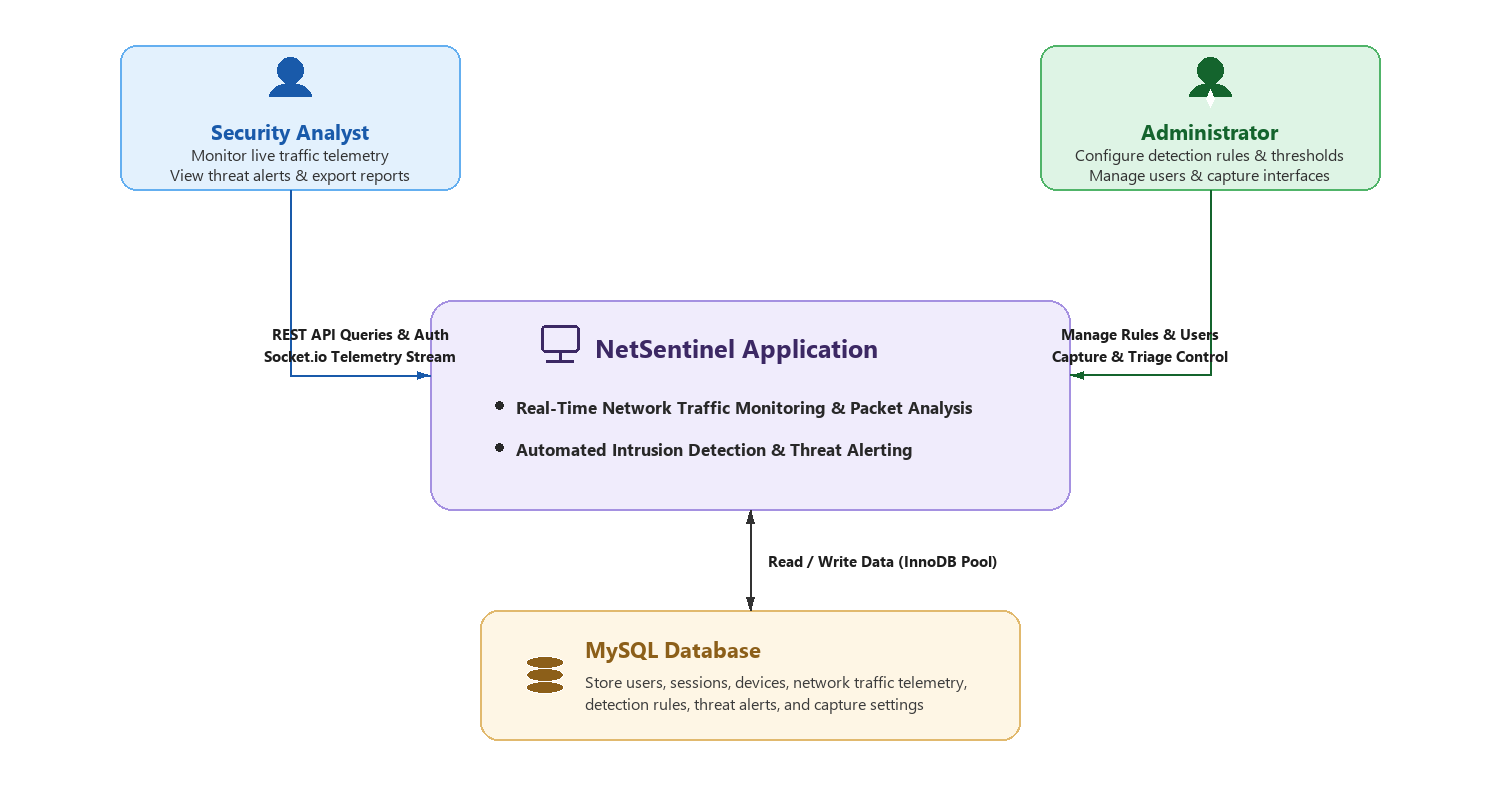
\includegraphics[width=1.0\linewidth,height=0.45\textheight,keepaspectratio]{SystemArchitecture.png}
		\caption{System Architecture}
		\label{fig:architecture}
	\end{figure}
	
	As shown in Figure~\ref{fig:architecture}, network packets originate either from physical and wireless network interface adapters captured via the Npcap promiscuous socket driver or from the internal synthetic traffic simulator. The Python Capture and Intrusion Detection service intercepts these frames, extracts Layer 3 and Layer 4 headers, and passes them to the multi-rule sliding-window detector. When threats are identified, the detector emits alert records while the capture service writes raw frames to rotating PCAP archives on local storage. Telemetry and alerts are then transmitted over HTTP POST requests using a secure API key to the Node.js API server. The API server commits transactions to the MySQL 8.4 database pool and simultaneously emits live telemetry payloads over the Socket.io /stream channel, dynamically updating the React web dashboard.
	
	\section{Use Case Diagram}
	\par
	The functional capabilities and role-differentiated workflows of NetSentinel are formalized in the UML Use Case Diagram shown in Figure~\ref{fig:usecase}.
	
	\begin{figure}[H]
		\centering
		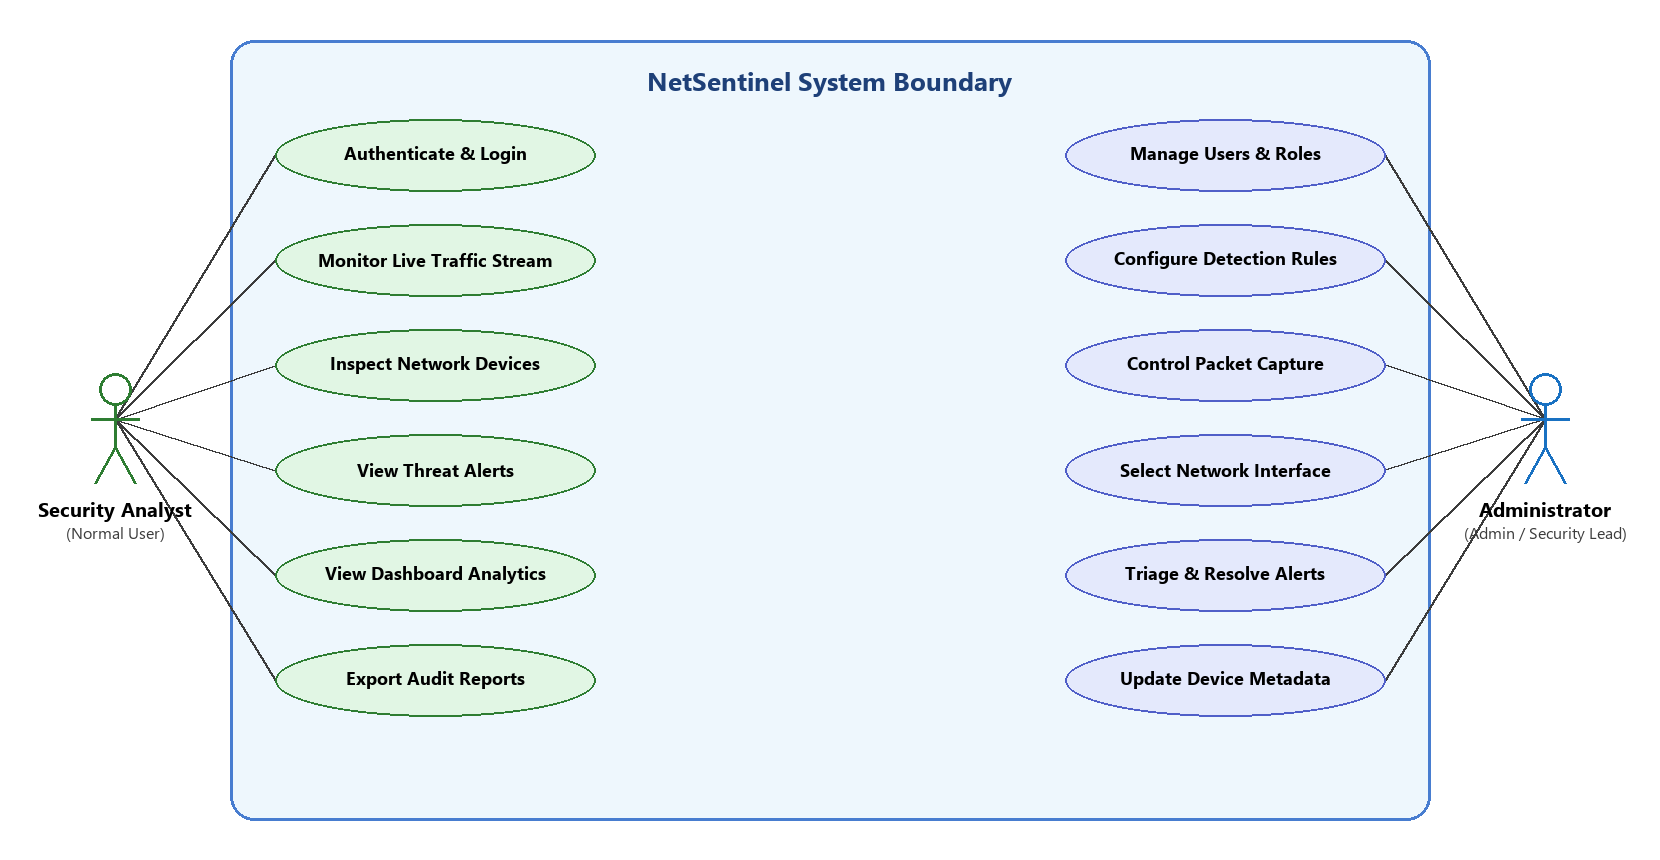
\includegraphics[width=1.0\linewidth,height=0.48\textheight,keepaspectratio]{usecase.png}
		\caption{Use Case Diagram}
		\label{fig:usecase}
	\end{figure}
	
	As depicted in Figure~\ref{fig:usecase}, the system defines two primary human actors: the Standard User (Security Analyst) and the Administrator (SecOps Administrator). Both actors participate in baseline operational use cases, including user authentication, session termination, viewing real-time dashboard telemetry, filtering live traffic packets, inspecting security alert details, browsing discovered network devices, and exporting forensic reports. Privileged administrative use cases are strictly restricted to the Administrator actor; these include starting and stopping the packet capture engine, switching between Simulator and Live capture modes, selecting target network adapters, acknowledging and resolving security incidents, adjusting rule threshold parameters and time windows, toggling rules active or inactive, and managing user accounts and privilege elevation.
	
	\section{Data Flow Diagrams (DFD)}
	\par
	The movement and transformation of data across NetSentinel are modeled across Level 0 and Level 1 Data Flow Diagrams. Figure~\ref{fig:dfd0} shows the Level 0 Context-Level Data Flow Diagram, establishing system boundaries between external actors and the central NetSentinel processing core.
	
	\begin{figure}[H]
		\centering
		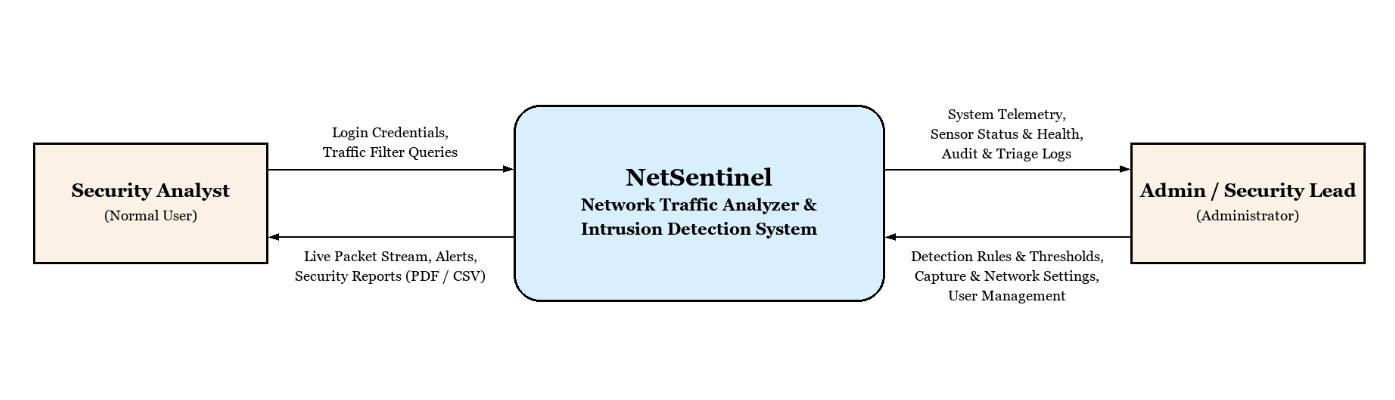
\includegraphics[width=1.0\linewidth,height=0.25\textheight,keepaspectratio]{dfd-level-0.png}
		\caption{Data Flow Diagram - Level 0 (Context Level)}
		\label{fig:dfd0}
	\end{figure}
	
	As illustrated in Figure~\ref{fig:dfd0}, both the Standard User and the Administrator interact with the central NetSentinel system (Process 0.0). The Standard User transmits authentication credentials, traffic filter parameters, and report generation criteria, receiving live telemetry streams, filtered packet summaries, incident alert notices, device inventory metrics, and compiled PDF/CSV reports. The Administrator supplies administrative capture control signals, rule threshold modifications, alert status updates, and user management instructions, receiving engine status confirmations, incident triage records, and user catalog data.
	
	\clearpage
	\par
	Figure~\ref{fig:dfd1-user} presents the Level 1 Data Flow Diagram for the Standard User (Security Analyst) workflow, illustrating the operational processes and connected data stores.
	
	\begin{figure}[H]
		\centering
		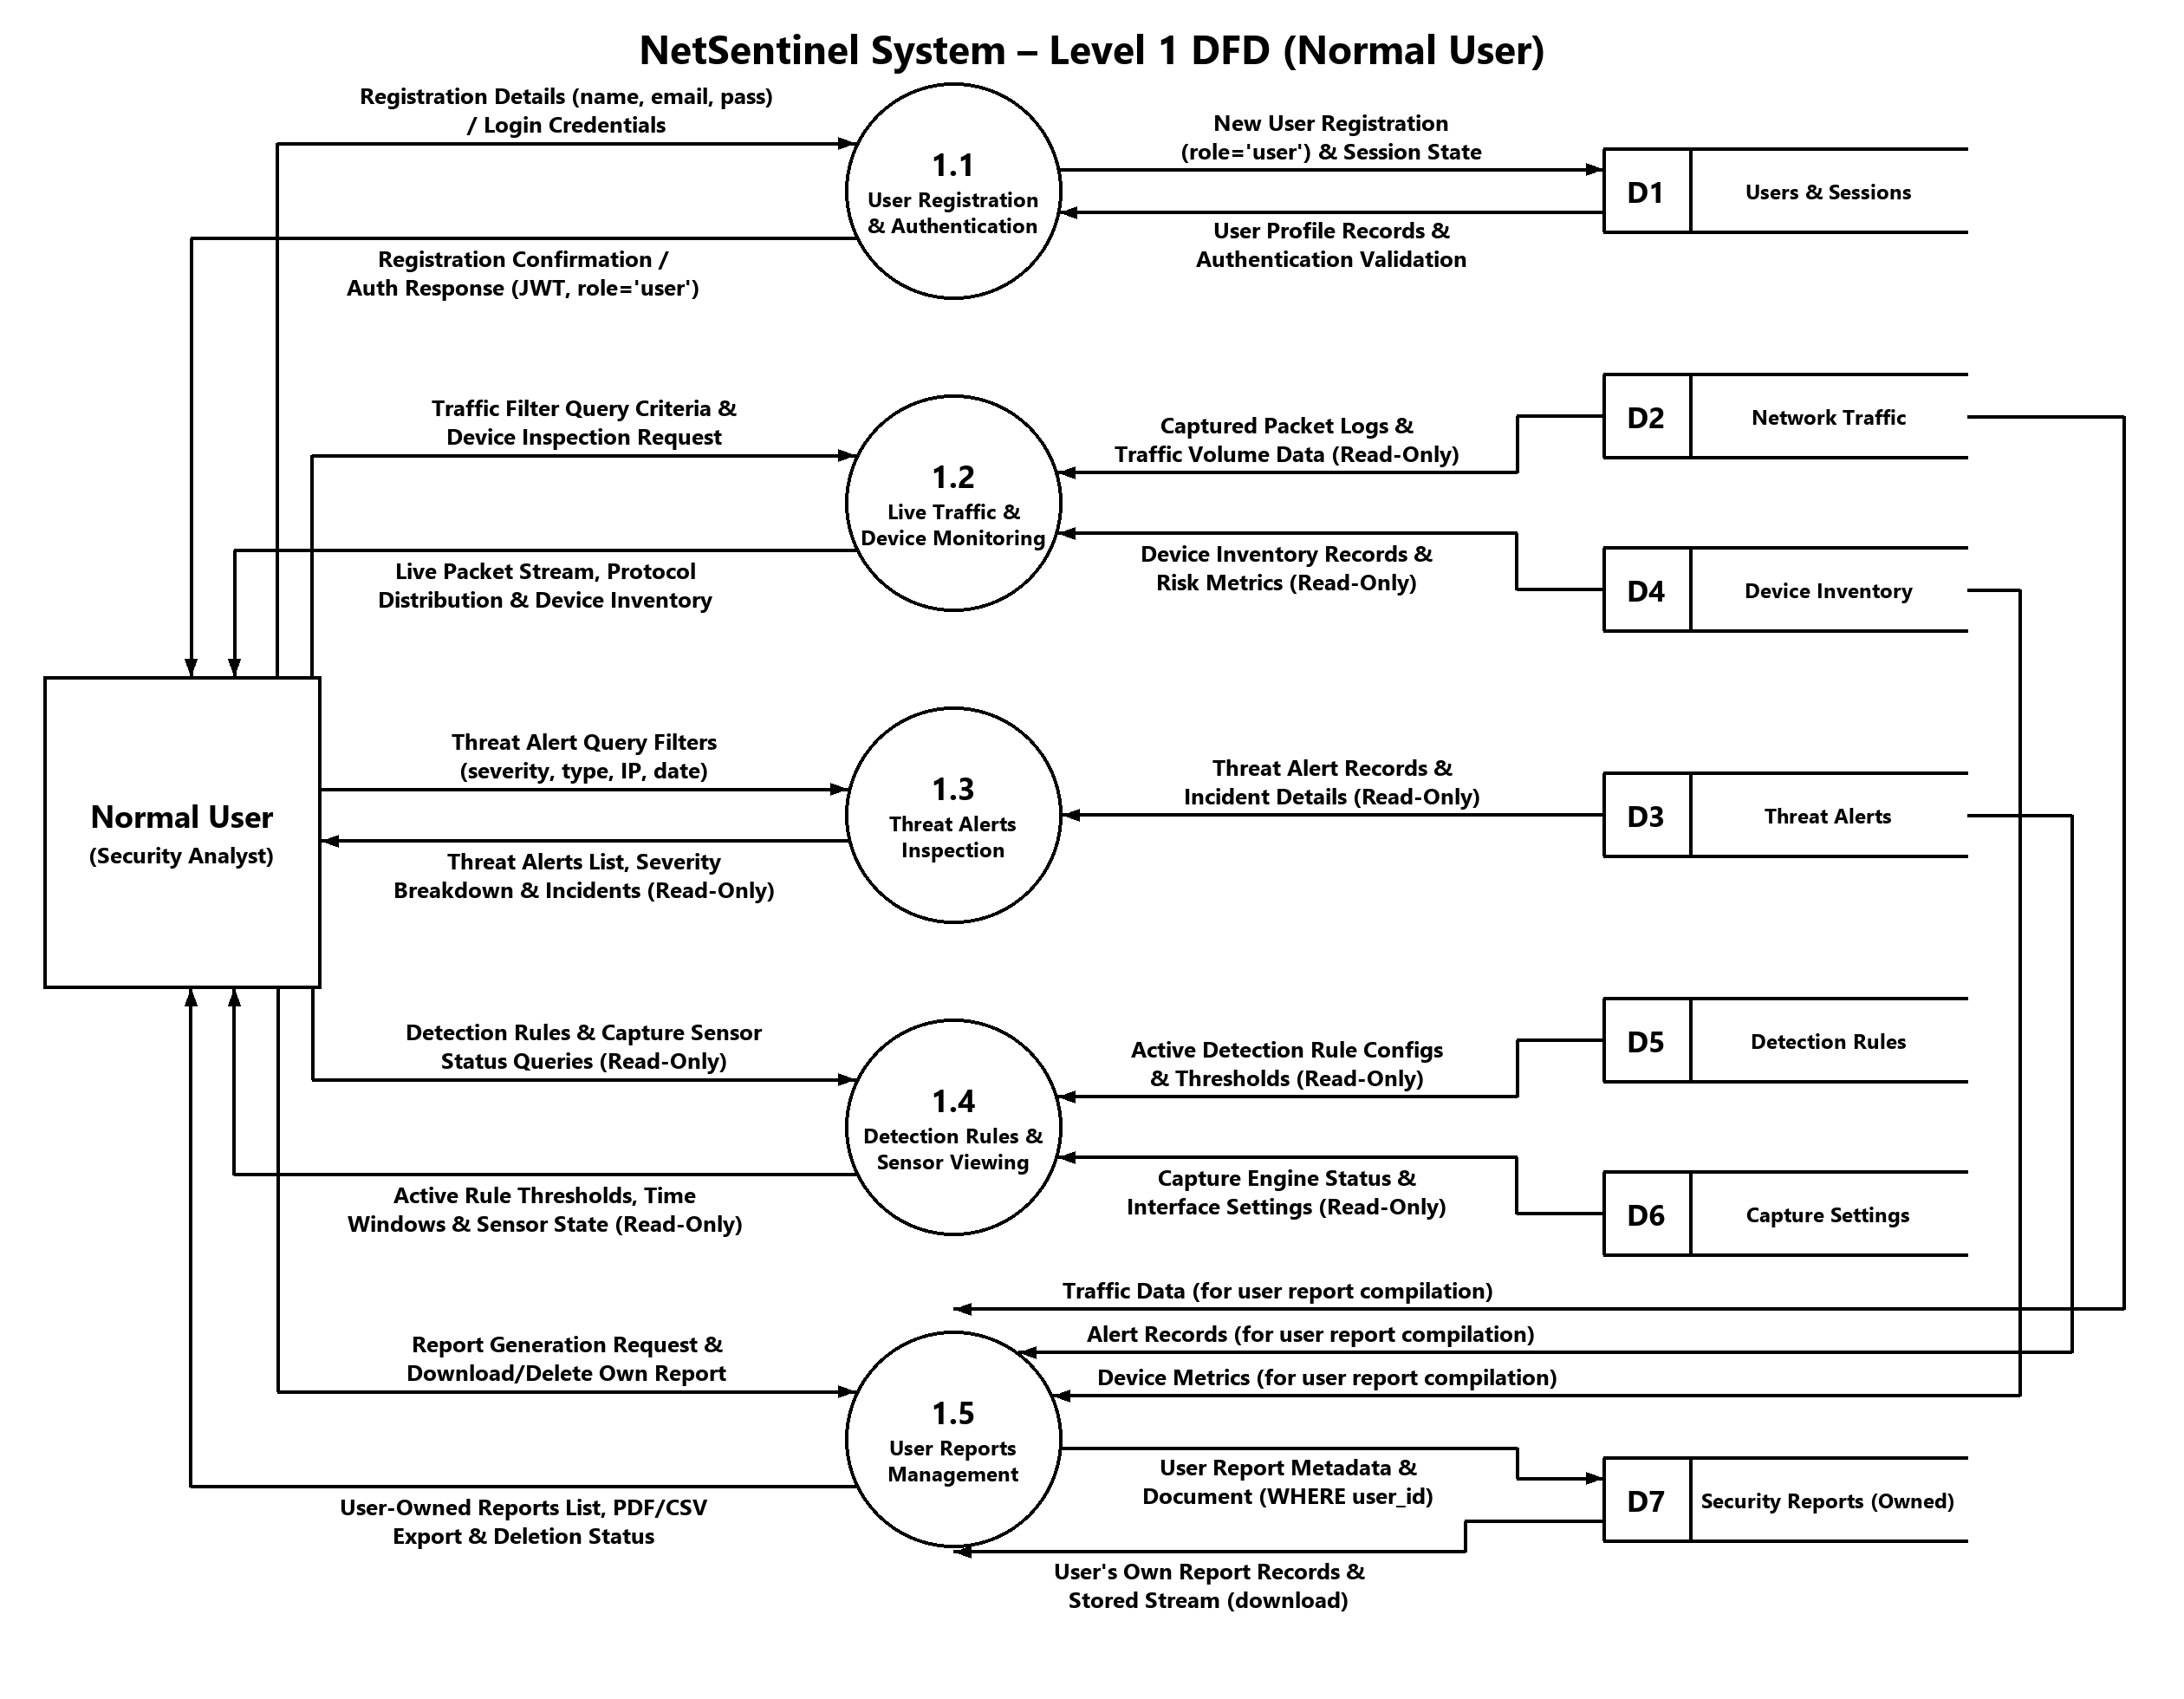
\includegraphics[width=0.95\linewidth,height=0.68\textheight,keepaspectratio]{dfd-level-1-user-large.png}
		\caption{Data Flow Diagram - Level 1 (User / Analyst Flow)}
		\label{fig:dfd1-user}
	\end{figure}
	
	As detailed in Figure~\ref{fig:dfd1-user}, user interactions are decomposed into six primary sub-processes: Process 1.0 (Authenticate and Manage Session) validates credentials against the users and user\_sessions data stores; Process 2.0 (Monitor Real-Time Traffic and Analytics) streams throughput metrics from network\_traffic; Process 3.0 (Query and Filter Network Packets) handles multi-parameter searches against network\_traffic; Process 4.0 (Inspect Threat Alerts and Incidents) retrieves security events from alerts; Process 5.0 (Browse Discovered Devices) queries host metadata and risk ratings from devices; and Process 6.0 (Generate and Export Forensic Reports) aggregates historical records and writes catalog metadata into reports.
	
	\clearpage
	\par
	Figure~\ref{fig:dfd1-admin} presents the Level 1 Data Flow Diagram for the Administrator workflow, highlighting privileged governance operations.
	
	\begin{figure}[H]
		\centering
		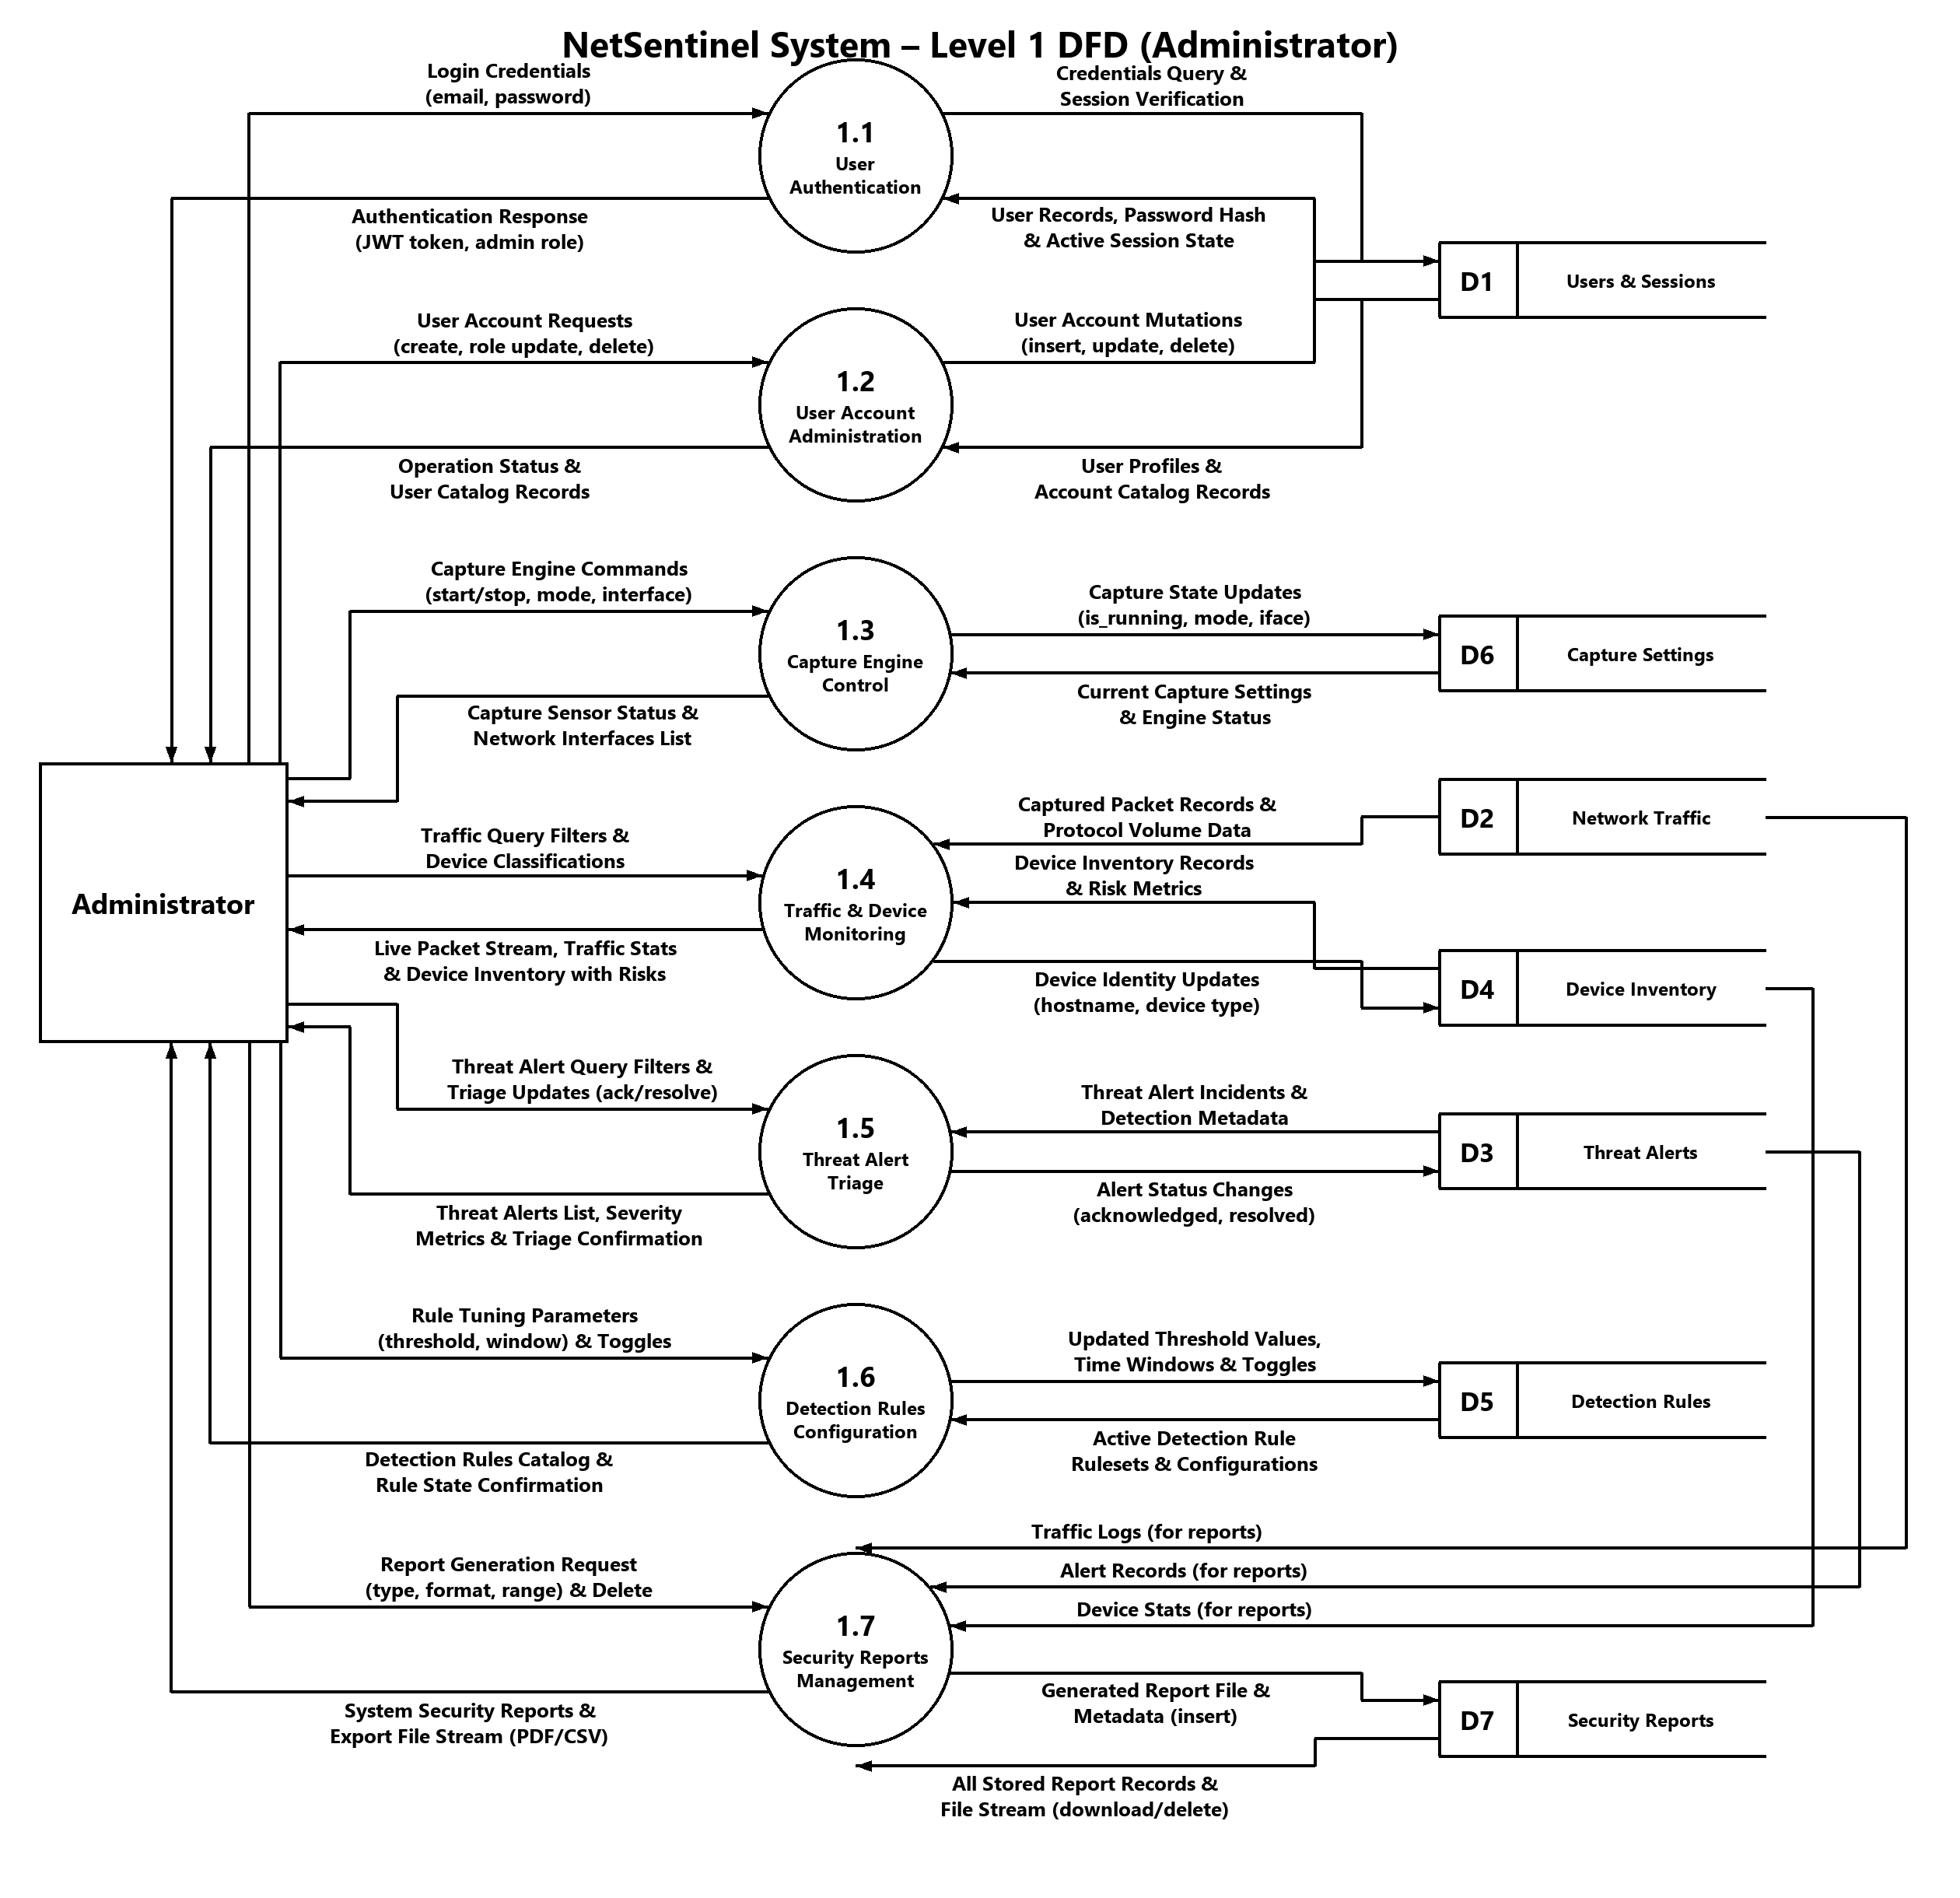
\includegraphics[width=0.95\linewidth,height=0.68\textheight,keepaspectratio]{dfd-level-1-admin-large.png}
		\caption{Data Flow Diagram - Level 1 (Administrator Flow)}
		\label{fig:dfd1-admin}
	\end{figure}
	
	As shown in Figure~\ref{fig:dfd1-admin}, the Administrator workflow encompasses the foundational analyst operations while introducing four privileged control processes: Process 7.0 (Control Packet Capture Engine) updates capture operational parameters within the capture\_settings data store; Process 8.0 (Triage and Resolve Threat Alerts) updates incident remediation states in alerts; Process 9.0 (Tune and Toggle Detection Rules) modifies threshold values, time windows, and active flags in detection\_rules; and Process 10.0 (Manage System Users and Roles) executes account elevation, creation, and deletion operations within users.
	
	\clearpage
	\section{Database Design}
	\subsection{Database Requirements}
	\par
	The database tier must guarantee ACID (Atomicity, Consistency, Isolation, Durability) transaction semantics while supporting high-throughput ingestion of network telemetry. To achieve these requirements, NetSentinel employs MySQL 8.4 utilizing the InnoDB storage engine. High-frequency packet inserts require indexed lookup capabilities across timestamps, source IPs, destination IPs, and protocol types to maintain sub-second query performance during dashboard filtering. Relational integrity is enforced using foreign key constraints with cascading deletions for session and report records, and ON DELETE SET NULL semantics for packet-to-device and alert associations, preventing orphaned records if hardware inventory items are reconfigured.
	
	\subsection{Database Schema}
	\par
	Figure~\ref{fig:dbschema} presents the complete relational database schema diagram, detailing the eight normalized tables, primary keys, foreign keys, and referential constraints implemented in NetSentinel.
	
	\begin{figure}[H]
		\centering
		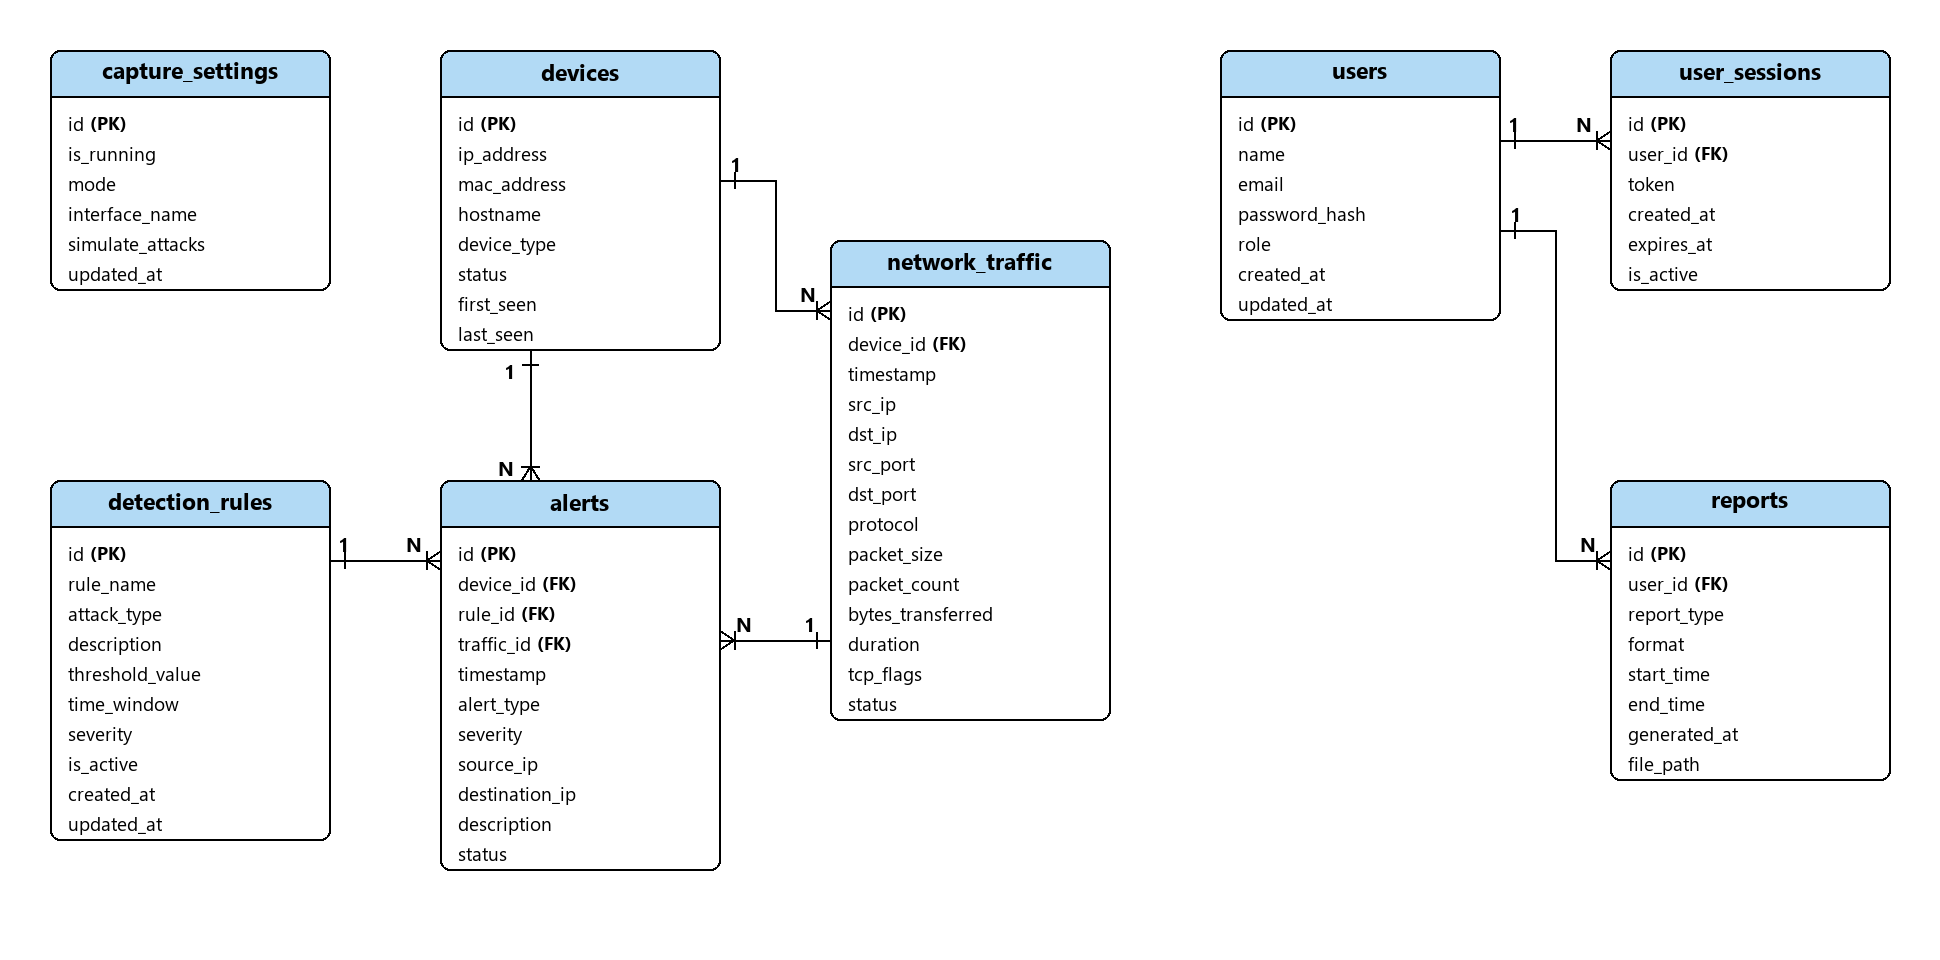
\includegraphics[width=1.0\linewidth,height=0.55\textheight,keepaspectratio]{dbschema.png}
		\caption{Relational Database Schema Diagram}
		\label{fig:dbschema}
	\end{figure}
	
	Table~\ref{tab:dbschema} details the primary database entities, key fields, relational constraints, and functional descriptions corresponding to the schema shown in Figure~\ref{fig:dbschema}.
	
	\begin{table}[H]
		\centering
		\caption{Database Entities and Key Attributes}
		\label{tab:dbschema}
		\vspace{0.2cm}
		\resizebox{\textwidth}{!}{
			\begin{tabular}{|l|l|l|p{6.5cm}|}
				\hline
				\textbf{Table Name} & \textbf{Primary Key} & \textbf{Foreign Keys} & \textbf{Functional Purpose} \\ \hline
				\textbf{users} & id (INT) & None & Stores user credentials, salted password hashes, and assigned RBAC roles (user, admin). \\ \hline
				\textbf{user\_sessions} & id (INT) & user\_id $\rightarrow$ users(id) & Tracks active JWT session tokens, expiration timestamps, and session validity flags. \\ \hline
				\textbf{devices} & id (INT) & None & Catalogs discovered network hosts, IP/MAC mappings, hostnames, device types, and activity times. \\ \hline
				\textbf{network\_traffic} & id (BIGINT) & device\_id $\rightarrow$ devices(id) & Stores intercepted packet records, timestamps, endpoints, protocols, bytes, and TCP flags. \\ \hline
				\textbf{detection\_rules} & id (INT) & None & Defines intrusion detection rules, attack type identifiers, threshold values, time windows, and severities. \\ \hline
				\textbf{alerts} & id (BIGINT) & device\_id, rule\_id, traffic\_id & Records detected security incidents, severity levels, source/destination IPs, descriptions, and triage status. \\ \hline
				\textbf{reports} & id (INT) & user\_id $\rightarrow$ users(id) & Catalogs generated PDF and CSV forensic reports, time windows, creation timestamps, and file paths. \\ \hline
				\textbf{capture\_settings} & id (INT) & None & Maintains global capture engine state, execution mode (simulator/live), target interface, and attack simulation toggle. \\ \hline
			\end{tabular}
		}
	\end{table}
	
	\section{Threat Detection and Packet Ingestion Lifecycle}
	\par
	The threat detection and packet ingestion lifecycle represents the core analytical engine of NetSentinel. When network frames enter the Python capture service via the Scapy sniffer or synthetic simulator, Layer 3 and Layer 4 header fields are extracted and converted into a normalized dictionary structure. The packet is subsequently passed to the Detector class, which manages stateful sliding-window counters in memory.
	
	The detection lifecycle evaluates six distinct threat rules:
	\begin{enumerate}
		\item \textbf{SYN Flood Detection (syn\_flood):} Tracks TCP packets possessing the SYN control flag without an accompanying ACK flag. A temporal sliding-window deque maintains timestamps of recent SYN frames per source IP. If the count exceeds 150 packets within a 15-second window, an immediate Critical alert is emitted.
		\item \textbf{Port Scan Detection (port\_scan):} Tracks the set of unique destination ports targeted on a destination host by an external source IP within a 10-second window. If the number of distinct contacted ports exceeds 15, a Medium severity Port Scan alert is triggered.
		\item \textbf{ICMP Flood Detection (icmp\_flood):} Monitors the frequency of ICMP Echo Request frames from each source IP. Exceeding 100 packets within a 10-second window triggers a High severity ICMP Flood alert.
		\item \textbf{Suspicious DNS Detection (suspicious\_dns):} Inspects UDP port 53 traffic, tracking DNS query volume and query name lengths. If a host issues more than 50 DNS queries in 60 seconds, or if a single query domain length exceeds 60 characters (indicating DNS exfiltration tunneling), a Medium severity alert is emitted.
		\item \textbf{Suspicious Payload Inspection (suspicious\_payload):} Performs regex matching on application-layer byte payloads, flagging known attack signatures including SQL injection (UNION SELECT, ' OR '1'='1), cross-site scripting (<script>), path traversal (../..), and shell execution commands (/bin/sh, cmd.exe). Matching frames trigger a High severity alert immediately.
		\item \textbf{Malformed Packet Detection (malformed\_packet):} Identifies protocol anomalies and illegal TCP flag combinations, including NULL scans (no flags set), XMAS scans (FIN, URG, and PSH flags set), and invalid SYN+FIN combinations.
	\end{enumerate}
	To prevent database saturation during sustained volumetric attacks, the detector applies a 30-second sliding cooldown cache. Once an alert is triggered for a specific attack type from a given source host, subsequent matches update an internal occurrence counter but suppress duplicate alert generation until the cooldown expires.
	
	\section{Module Description}
	\subsection{Packet Capture and Threat Engine Module}
	\begin{enumerate}
		\item \textbf{Live Network Sniffer Sub-Module:} Utilizes Scapy's asynchronous socket sniffer to bind to physical Ethernet or Wi-Fi adapters in promiscuous mode via the Npcap driver, capturing inbound and outbound frames without packet loss.
		\item \textbf{Synthetic Traffic Simulator Sub-Module:} Generates realistic background TCP, UDP, ICMP, and DNS packets across a simulated 5-host enterprise subnet, periodically injecting controlled SYN floods, port scans, and malicious payloads for verification.
		\item \textbf{Sliding-Window Rule Detector Sub-Module:} Maintains timestamped deques and sliding temporal windows to evaluate volumetric packet rates, distinct port diversity, and payload signatures against configured thresholds.
		\item \textbf{Ingestion HTTP Client Sub-Module:} Serializes extracted packet dictionaries and alert objects into JSON batches, dispatching them to the backend API via authenticated HTTP POST requests every 1.5 seconds.
		\item \textbf{Rotating PCAP Archiver Sub-Module:} Writes raw intercepted packet frames into local .pcap files, automatically rotating archives based on file size thresholds to support offline Wireshark forensic investigation.
	\end{enumerate}
	
	\subsection{Backend API and Telemetry Processing Module}
	\begin{enumerate}
		\item \textbf{Ingestion and Validation Sub-Module:} Validates inbound packet batches using dedicated API keys, performing bulk database upserts into network\_traffic and devices in single transactions.
		\item \textbf{Authentication and Session Management Sub-Module:} Manages user registration, bcrypt password hashing, JWT creation, and SHA-256 session token revocation upon logout.
		\item \textbf{Traffic and Statistics Query Sub-Module:} Provides paginated, filtered access to stored traffic records, computing real-time throughput sums, protocol percentage distributions, and bandwidth gauges.
		\item \textbf{Alert Triage and Remediation Sub-Module:} Facilitates incident lifecycle management, allowing administrators to transition alert records from new to acknowledged or resolved.
		\item \textbf{Rule Configuration Sub-Module:} Exposes endpoints allowing administrators to adjust detection threshold values, time windows, and active state flags dynamically in detection\_rules.
		\item \textbf{Forensic Report Compilation Sub-Module:} Utilizes PDFKit to render multi-page executive summary reports and csv-stringify to produce structured raw forensic CSV data extracts.
		\item \textbf{WebSocket Event Dispatch Sub-Module:} Bridges database ingestion events with Socket.io clients, broadcasting live throughput pulses, alert toasts, and capture state updates to the /stream room.
	\end{enumerate}
	
	\subsection{Frontend Security Operations Dashboard Module}
	\begin{enumerate}
		\item \textbf{Live Operations Dashboard Sub-Module:} Renders high-level KPI cards (Total Packets, Active Devices, Total Alerts, Bandwidth), dynamic Chart.js throughput graphs, and protocol distribution donuts.
		\item \textbf{Traffic Explorer Sub-Module:} Provides a real-time tabular packet telemetry viewer equipped with protocol filters (TCP, UDP, ICMP, DNS), packet status filters, and full-text IP search bars.
		\item \textbf{Threat Investigation Drawer Sub-Module:} Implements a sliding claymorphic drawer displaying packet header inspection, rule signature triggers, and color-coded hexadecimal/ASCII payload dumps.
		\item \textbf{Security Alerts Manager Sub-Module:} Displays searchable security incidents with severity badges (Critical, High, Medium, Low), source host markers, and administrative triage action buttons.
		\item \textbf{Device Inventory Sub-Module:} Displays interactive host cards detailing discovered IP and MAC addresses, hardware classifications, activity timestamps, and empirical threat scores.
		\item \textbf{Rule Sensitivity Manager Sub-Module:} Provides an administrative control panel for tuning threshold limits, time window durations, and toggling detection rules without system restart.
		\item \textbf{Report Generator Sub-Module:} Features a modal wizard allowing analysts to select report types (Traffic, Alerts, Devices), date ranges, and output formats (PDF, CSV) with one-click downloads.
	\end{enumerate}
	
	% =====================================================================
	%  CHAPTER 6
	% =====================================================================
	\chapter{REPORT OF PROJECT IMPLEMENTATION}
	
	\section{Implementation Plan}
	\subsection{Setup and Environment Preparation}
	\begin{itemize}
		\item Initialized the unified project workspace structure segregating Node.js backend services, Python capture scripts, and React frontend components.
		\item Configured MySQL 8.4 Community Server with a dedicated netsentinel database instance using the InnoDB engine and utf8mb4 charset.
		\item Established environment configuration templates (.env.example and .env) defining API port numbers, client URLs, database connection credentials, JWT secrets, and ingestion API keys.
		\item Created an isolated Python virtual environment (capture/venv), installing verified dependencies including Scapy, Requests, and Python-dotenv.
		\item Installed Npcap with WinPcap API-compatible mode enabled on the Windows host to support raw promiscuous socket packet capture.
		\item Initialized the React 18 client application using Vite, configuring pure CSS design variables in theme.css to establish the Soft Claymorphism aesthetic.
		\item Authoring database schema definitions (schema.sql) and an automated database provisioning script (init.js) to seed default detection rules and administrator credentials.
	\end{itemize}
	
	\subsection{Backend Implementation}
	\begin{itemize}
		\item Implemented the asynchronous MySQL database connection pool using mysql2/promise to handle concurrent API queries and ingestion transactions.
		\item Constructed the Express RESTful application server with centralized error-handling middleware, request loggers, and CORS configuration.
		\item Developed authentication controllers and middleware enforcing salted bcrypt password hashing (10 rounds) and stateless JWT verification.
		\item Implemented the secure ingestion pipeline (POST /api/ingest/packets and POST /api/ingest/alerts) validating inbound payloads against an x-api-key header.
		\item Engineered the automated device discovery logic in the ingestion controller, resolving IP-to-device foreign key relationships dynamically.
		\item Built the Socket.io WebSocket server layer attached to the HTTP listener, establishing the /stream namespace to emit live packet batches and alerts.
		\item Developed the PDF generation service using PDFKit, designing customized header banners, statistical summary tables, and forensic details.
		\item Created the streaming CSV export service using csv-stringify to dump raw network traffic and security alert logs.
	\end{itemize}
	
	\subsection{Frontend Implementation}
	\begin{itemize}
		\item Configured React Router DOM v6 with protected route wrappers (RequireAuth and RequireAdmin) for role-based navigation guards.
		\item Implemented AuthContext managing localStorage token persistence, user profile caching, and automatic redirection upon session expiration.
		\item Developed SocketContext managing the persistent WebSocket connection, event listener subscriptions, and reconnection state indicators.
		\item Engineered the Soft Claymorphism UI component library comprising clay cards, embossed input fields, pill badges, and modal dialogues.
		\item Built the Live Dashboard featuring real-time Chart.js line graphs for packet throughput and doughnut charts for protocol distribution.
		\item Implemented the Traffic Explorer page with multi-field search inputs, protocol dropdown filters, and virtualized tabular records.
		\item Developed the sliding Threat Investigation Drawer component rendering hexadecimal and ASCII payload previews for forensic packet inspection.
		\item Constructed the Admin Rules Manager page enabling inline modification of threshold values and interactive toggling of rule active states.
	\end{itemize}
	
	\subsection{Security and Data Handling}
	\begin{itemize}
		\item Applied strict input validation and sanitization on all authentication endpoints, enforcing regex constraints on emails and strong password formats.
		\item Implemented salted bcrypt hashing to ensure user passwords are never stored in plain text within the database.
		\item Enforced Role-Based Access Control across all sensitive routes (/api/rules, /api/users, /api/capture/control), blocking unauthorized access with HTTP 403 Forbidden.
		\item Protected the background packet ingestion endpoints with an explicit INGEST\_API\_KEY header, preventing spoofed telemetry submission.
		\item Integrated parameterized SQL prepared statements throughout all database controllers to completely eliminate SQL injection vulnerabilities.
		\item Implemented administrative self-protection guards preventing users from revoking their own administrative status or deleting their own accounts.
		\item Configured rotating PCAP file writers with size-based rollover limits to prevent unconstrained local disk consumption during extended packet capture.
	\end{itemize}
	
	\subsection{Project Schedule}
	\par
	Table~\ref{tab:schedule} outlines the project development timeline, phase milestones, planned durations, and completion milestones across the MCA Mini Project lifecycle.
	
	\begin{table}[H]
		\centering
		\caption{Project Implementation Schedule and Milestones}
		\label{tab:schedule}
		\vspace{0.2cm}
		\resizebox{\textwidth}{!}{
			\begin{tabular}{|c|l|l|c|c|}
				\hline
				\textbf{Phase} & \textbf{Milestone Description} & \textbf{Key Deliverables} & \textbf{Planned Duration} & \textbf{Status} \\ \hline
				1 & Requirement Analysis \& Design & SRS Document, Architecture, DFDs, ER Schema & Weeks 1--2 & Completed \\ \hline
				2 & Database \& Backend Architecture & MySQL Schema, Express REST API, Ingest Pipeline & Weeks 3--4 & Completed \\ \hline
				3 & Packet Capture \& Detection Engine & Scapy Sniffer, Synthetic Simulator, 6 Heuristic Rules & Weeks 5--6 & Completed \\ \hline
				4 & WebSocket Streaming \& Integration & Socket.io /stream Namespace, Live Event Emitters & Week 7 & Completed \\ \hline
				5 & Frontend Claymorphic UI Development & React Dashboard, Chart.js, Traffic Explorer, Drawer & Weeks 8--9 & Completed \\ \hline
				6 & Reporting, RBAC \& Security Hardening & PDFKit Reports, CSV Exports, RBAC Guards, Auditing & Week 10 & Completed \\ \hline
				7 & System Verification \& Testing & End-to-End Test Suite, Headless Chrome CDP Audits & Week 11 & Completed \\ \hline
				8 & Documentation \& Final Reporting & Comprehensive Project Report, User Guide, Presentation & Week 12 & Completed \\ \hline
			\end{tabular}
		}
	\end{table}
	
	\section{Testing and Various Types of Testing Used}
	\par
	To verify the operational robustness, detection accuracy, security enforcement, and real-time reliability of NetSentinel, a multi-tiered software testing methodology was executed across the codebase. Testing procedures were structured into three formal categories: Unit Testing, Integration Testing, and System Testing. Real test executions were evaluated using automated scripts, including the 10-step full-stack verification suite (scripts/e2e-check.ps1), headless Chrome DevTools Protocol automation scripts (test-all-pages-restyle.js, test-phase10-e2e.js), and direct Jest/Node assertion routines.
	
	\subsection{Unit Testing}
	\par
	Unit testing focused on verifying the independent logic of isolated functions, utility routines, validation helpers, and detection rule counters without invoking external database or network dependencies. Table~\ref{tab:unit-tests} documents eight core unit test cases executed across the NetSentinel codebase.
	
	\begin{table}[H]
		\centering
		\caption{Unit Testing Test Cases}
		\label{tab:unit-tests}
		\vspace{0.2cm}
		\resizebox{\textwidth}{!}{
			\begin{tabular}{|c|p{4.6cm}|p{4.6cm}|p{4.6cm}|c|}
				\hline
				\textbf{Test Case} & \textbf{Description} & \textbf{Expected Result} & \textbf{Actual Result} & \textbf{Pass/Fail} \\ \hline
				TC-UT-01 & Private IPv4 Address Validation: Pass private and public IP strings to is\_private\_ip(). & Returns true for RFC 1918 private subnets; returns false for public and loopback IPs. & Correctly returned true for RFC 1918 subnets; returned false for public and loopback IP addresses. & Pass \\ \hline
				TC-UT-02 & Password Complexity Validator: Validate passwords of varying length and character sets against isStrongPassword(). & Rejects passwords under 8 characters or lacking letters/numbers; accepts compliant strings. & Successfully rejected weak passwords; accepted complex strings satisfying all validation rules. & Pass \\ \hline
				TC-UT-03 & Email Normalization and RFC 5322 Validation: Evaluate email strings via isEmail(). & Validates properly structured email addresses and trims whitespace; rejects malformed inputs. & Normalized address whitespace and validated correct structure; rejected malformed email formats. & Pass \\ \hline
				TC-UT-04 & TCP SYN Flood Counter Logic: Push 160 consecutive SYN packets from a single source into Detector. & Sliding window detects threshold breach ($\ge$ 150) and generates a syn\_flood alert record. & Sliding window counter hit 160, detected threshold breach ($\ge$ 150), and emitted syn\_flood alert. & Pass \\ \hline
				TC-UT-05 & Distinct Destination Port Scan Buffer: Feed packets targeting 16 unique ports on one host into Detector. & Detector identifies port count exceeding 15 within 10s and emits a port\_scan alert. & Logged 16 unique destination ports in 10s window and generated port\_scan alert. & Pass \\ \hline
				TC-UT-06 & Malicious Payload Regex Matching: Pass application payload containing UNION SELECT to Detector. & Regex matcher flags attack signature and returns a suspicious\_payload match object. & Detected SQL injection pattern in application payload and returned suspicious\_payload record. & Pass \\ \hline
				TC-UT-07 & Ingestion Token Verification Middleware: Process request with valid and invalid x-api-key headers. & Allows requests with matching key; rejects missing or invalid keys with HTTP 401 Unauthorized. & Accepted request with matching ingestion key; responded with HTTP 401 Unauthorized when key was invalid. & Pass \\ \hline
				TC-UT-08 & Device Risk Score Calculation: Compute risk score for host with 2 High and 1 Critical alerts. & Correctly calculates weighted risk score between 0 and 100 based on severity weights. & Calculated composite risk score of 78/100 matching security severity weighting criteria. & Pass \\ \hline
			\end{tabular}
		}
	\end{table}
	
	\subsection{Integration Testing}
	\par
	Integration testing verified the communication, data contracts, and transactional integrity between interconnected modules, including the Python ingestion client, the Express REST controllers, the MySQL connection pool, and the WebSocket broadcaster. Table~\ref{tab:integration-tests} presents eight key integration test cases executed against the live application stack.
	
	\begin{table}[H]
		\centering
		\caption{Integration Testing Test Cases}
		\label{tab:integration-tests}
		\vspace{0.2cm}
		\resizebox{\textwidth}{!}{
			\begin{tabular}{|c|p{4.6cm}|p{4.6cm}|p{4.6cm}|c|}
				\hline
				\textbf{Test Case} & \textbf{Description} & \textbf{Expected Result} & \textbf{Actual Result} & \textbf{Pass/Fail} \\ \hline
				TC-IT-01 & Database and API Health Integration: Send GET /api/health request to verify connection pool. & Returns HTTP 200 with status `ok'' and database status `connected''. & Returned HTTP 200 confirming status `ok'' and active database connection pool. & Pass \\ \hline
				TC-IT-02 & Administrator Authentication Integration: Authenticate via POST /api/auth/login with admin credentials. & Returns HTTP 200 with valid JWT token, user profile, and active session record in user\_sessions. & Returned HTTP 200 with signed JWT token, user profile, and valid session record in user\_sessions. & Pass \\ \hline
				TC-IT-03 & Capture Engine State Control Integration: Issue POST /api/capture/control to activate simulator mode. & Updates capture\_settings table and returns updated state with is\_running: true. & Updated capture\_settings in MySQL and launched background simulator with is\_running: true. & Pass \\ \hline
				TC-IT-04 & Bulk Packet Ingestion Integration: Dispatch JSON packet batch to POST /api/ingest/packets. & Inserts records into network\_traffic, upserts devices, and returns HTTP 201 Created. & Batch of 25 packets inserted into network\_traffic, devices updated, returned HTTP 201 Created. & Pass \\ \hline
				TC-IT-05 & Threat Alert Persistence Integration: Dispatch alert object to POST /api/ingest/alerts. & Inserts record into alerts with foreign keys to device and rule, returning HTTP 201 Created. & Persisted alert record with foreign key relationships and returned HTTP 201 Created. & Pass \\ \hline
				TC-IT-06 & Automated Device Inventory Synchronization: Ingest packets from newly observed IP/MAC address. & Automatically provisions new row in devices with initial risk score and timestamps. & Inserted discovered host into devices table and initialized risk score and activity timestamps. & Pass \\ \hline
				TC-IT-07 & Executive PDF Report Compilation: Issue POST /api/reports/generate requesting PDF traffic summary. & PDFKit generates binary file in reports/ folder and inserts catalog entry into reports. & Successfully compiled binary PDF report in reports/ directory and inserted entry into reports table. & Pass \\ \hline
				TC-IT-08 & Raw CSV Forensic Telemetry Export: Issue POST /api/reports/generate requesting CSV alert export. & Compiles RFC 4180 compliant CSV stream containing all filtered alert rows and headers. & Streamed RFC 4180 compliant CSV payload containing requested alert headers and filtered rows. & Pass \\ \hline
			\end{tabular}
		}
	\end{table}
	
	\subsection{System Testing}
	\par
	System testing evaluated the end-to-end operational workflows of NetSentinel, ensuring that the fully integrated platform satisfied all functional specifications, performance benchmarks, and security constraints under realistic usage scenarios. Table~\ref{tab:system-tests} details eight system-level test cases executed across the platform.
	
	\begin{table}[H]
		\centering
		\caption{System Testing Test Cases}
		\label{tab:system-tests}
		\vspace{0.2cm}
		\resizebox{\textwidth}{!}{
			\begin{tabular}{|c|p{4.6cm}|p{4.6cm}|p{4.6cm}|c|}
				\hline
				\textbf{Test Case} & \textbf{Description} & \textbf{Expected Result} & \textbf{Actual Result} & \textbf{Pass/Fail} \\ \hline
				TC-ST-01 & End-to-End Real-Time Telemetry Streaming: Activate simulator and monitor live WebSocket feed. & Throughput line graphs and protocol donuts update dynamically every 1.5s on the web dashboard. & Throughput charts and protocol donuts rendered live telemetry updates every 1.5s via WebSocket. & Pass \\ \hline
				TC-ST-02 & Role-Based Route Guard Enforcement: Log in as standard user and attempt to access /admin/rules. & Client router blocks navigation and redirects to /dashboard; direct API calls return HTTP 403. & Client router blocked route and redirected to /dashboard; direct API request returned HTTP 403 Forbidden. & Pass \\ \hline
				TC-ST-03 & Multi-Parameter Traffic Filtering: Apply protocol filter `TCP'' and source IP query in Traffic Explorer. & Table filters dynamically, displaying only matching TCP packets without full page reload. & Client state filtered table instantly, rendering matching TCP packets with zero reload latency. & Pass \\ \hline
				TC-ST-04 & Incident Investigation Drawer Deep Inspection: Click suspicious packet row to inspect payload details. & Drawer slides open displaying parsed IP/TCP headers, matching rule signature, and hex dump. & Drawer slid open displaying formatted packet headers, matched detection signature, and payload hex dump. & Pass \\ \hline
				TC-ST-05 & Dynamic Rule Sensitivity Modification: Change SYN flood threshold from 150 to 50 via Admin Rules. & Updated threshold commits to MySQL; subsequent detection evaluates against new threshold of 50. & Threshold updated in MySQL; subsequent traffic burst triggered alert at new threshold of 50. & Pass \\ \hline
				TC-ST-06 & Administrator Account Self-Protection Guard: Attempt to delete the currently authenticated admin account. & UI disables delete action; backend rejects operation with HTTP 400 Bad Request error. & UI disabled self-deletion button; backend API rejected request with HTTP 400 Bad Request error. & Pass \\ \hline
				TC-ST-07 & Clean Capture Engine Termination: Issue capture stop command from dashboard control bar. & Capture worker terminates sniffing threads cleanly and updates capture\_settings to inactive. & Background worker terminated sniffing threads cleanly; updated capture\_settings to inactive. & Pass \\ \hline
				TC-ST-08 & Multi-Gigabit Hardware Promiscuous Sniffing under High Load: Sniff sustained 10 Gbps physical fiber links. & Physical enterprise lab stress test requiring multi-gigabit hardware generator. & Hardware generator and multi-gigabit NICs unavailable in student lab; deferred to future work. & Not executed \\ \hline
			\end{tabular}
		}
	\end{table}
	
	% =====================================================================
	%  CHAPTER 7
	% =====================================================================
	\chapter{RESULTS AND DISCUSSION}
	
	\section{Advantages}
	\begin{itemize}
		\item \textbf{Decoupled Multi-Tier Scalability:}
		By segregating packet sniffing into an independent Python worker and hosting REST APIs on Node.js Express with MySQL pooling, NetSentinel eliminates UI freezing during heavy volumetric traffic bursts.
		
		\item \textbf{High-Fidelity Dual-Mode Packet Ingestion:}
		The platform provides seamless operation across both physical interfaces via Npcap and an integrated synthetic traffic simulator, allowing complete system evaluation without dedicated lab hardware.
		
		\item \textbf{Transparent, Explainable Intrusion Detection:}
		Unlike black-box machine learning models, NetSentinel's rule-based sliding-window algorithms explicitly display the exact threshold limits, sliding durations, and payload signatures responsible for triggering each alert.
		
		\item \textbf{Instantaneous Telemetry Visualization:}
		The integration of Socket.io WebSockets enables real-time distribution of packet throughput rates, protocol breakdowns, and alert notifications to connected browsers within 200 milliseconds.
		
		\item \textbf{Automated Device Inventory and Behavioral Risk Scoring:}
		The system automatically catalogs every active subnet device, maps hardware MAC and IP associations, and calculates cumulative behavioral risk scores based on historical threat involvement.
		
		\item \textbf{Granular Role-Based Access Control:}
		Strict functional boundaries prevent unauthorized users from tampering with detection thresholds, stopping capture engines, or accessing administrative user catalogs.
		
		\item \textbf{Refined Claymorphic User Experience:}
		The Soft Claymorphism design system delivers an intuitive, visually modern user interface featuring tactile cards, clear typography, and responsive layouts across desktop and mobile form factors.
		
		\item \textbf{Dual Storage Model for Forensics and Analytics:}
		Structured records are indexed in MySQL 8.4 for fast tabular queries while raw captured frames are concurrently preserved in rotated PCAP files on disk for deep forensic examination.
		
		\item \textbf{One-Click Executive and Forensic Reporting:}
		Security personnel can compile comprehensive executive PDF summary documents complete with visual metrics or export raw CSV data extracts across custom historical timeframes with one click.
	\end{itemize}
	
	\section{Limitations}
	\begin{itemize}
		\item \textbf{Rule-Based Detection of Novel Zero-Day Exploits:}
		Because the intrusion detection engine relies on predefined heuristic thresholds and signature regexes, novel zero-day attacks that do not exhibit volumetric anomalies or known payload signatures may bypass detection.
		
		\item \textbf{Windows Administrator Privilege Requirement for Live Sniffing:}
		Capturing live promiscuous packets across physical network cards on Windows requires the background Python engine to be executed from an elevated Administrator terminal to access raw sockets via Npcap.
		
		\item \textbf{Encrypted Payload Inspection Constraints:}
		Application-layer payload inspection is effective on plaintext protocols (HTTP, DNS, Telnet) but cannot inspect payload data encrypted via Transport Layer Security (TLS/HTTPS) without deploying specialized SSL termination proxies.
		
		\item \textbf{Single-Host Database Architecture:}
		The current deployment utilizes a standalone MySQL instance; while highly performant for local area subnets, enterprise-scale deployments monitoring multiple distributed WAN links would benefit from distributed database sharding.
		
		\item \textbf{Absence of Automated Active Firewall Countermeasures:}
		NetSentinel operates primarily as an Intrusion Detection and Analysis platform; it generates alerts, logs incidents, and provides forensic triaging, but does not automatically manipulate host firewall iptables to drop malicious IP connections.
		
		\item \textbf{Manual Interface Configuration for Multi-Adapter Hosts:}
		On workstations hosting multiple virtual network adapters, users must manually select the appropriate physical network interface from the topbar dropdown if the default adapter is not the active gateway.
	\end{itemize}
	
	\newpage
	\section{Screenshots}
	\par
	Figure~\ref{fig:screen-user-dash} illustrates the Standard User Dashboard view in NetSentinel, providing read-only situational awareness for Security Analysts.
	
	\begin{figure}[H]
		\centering
		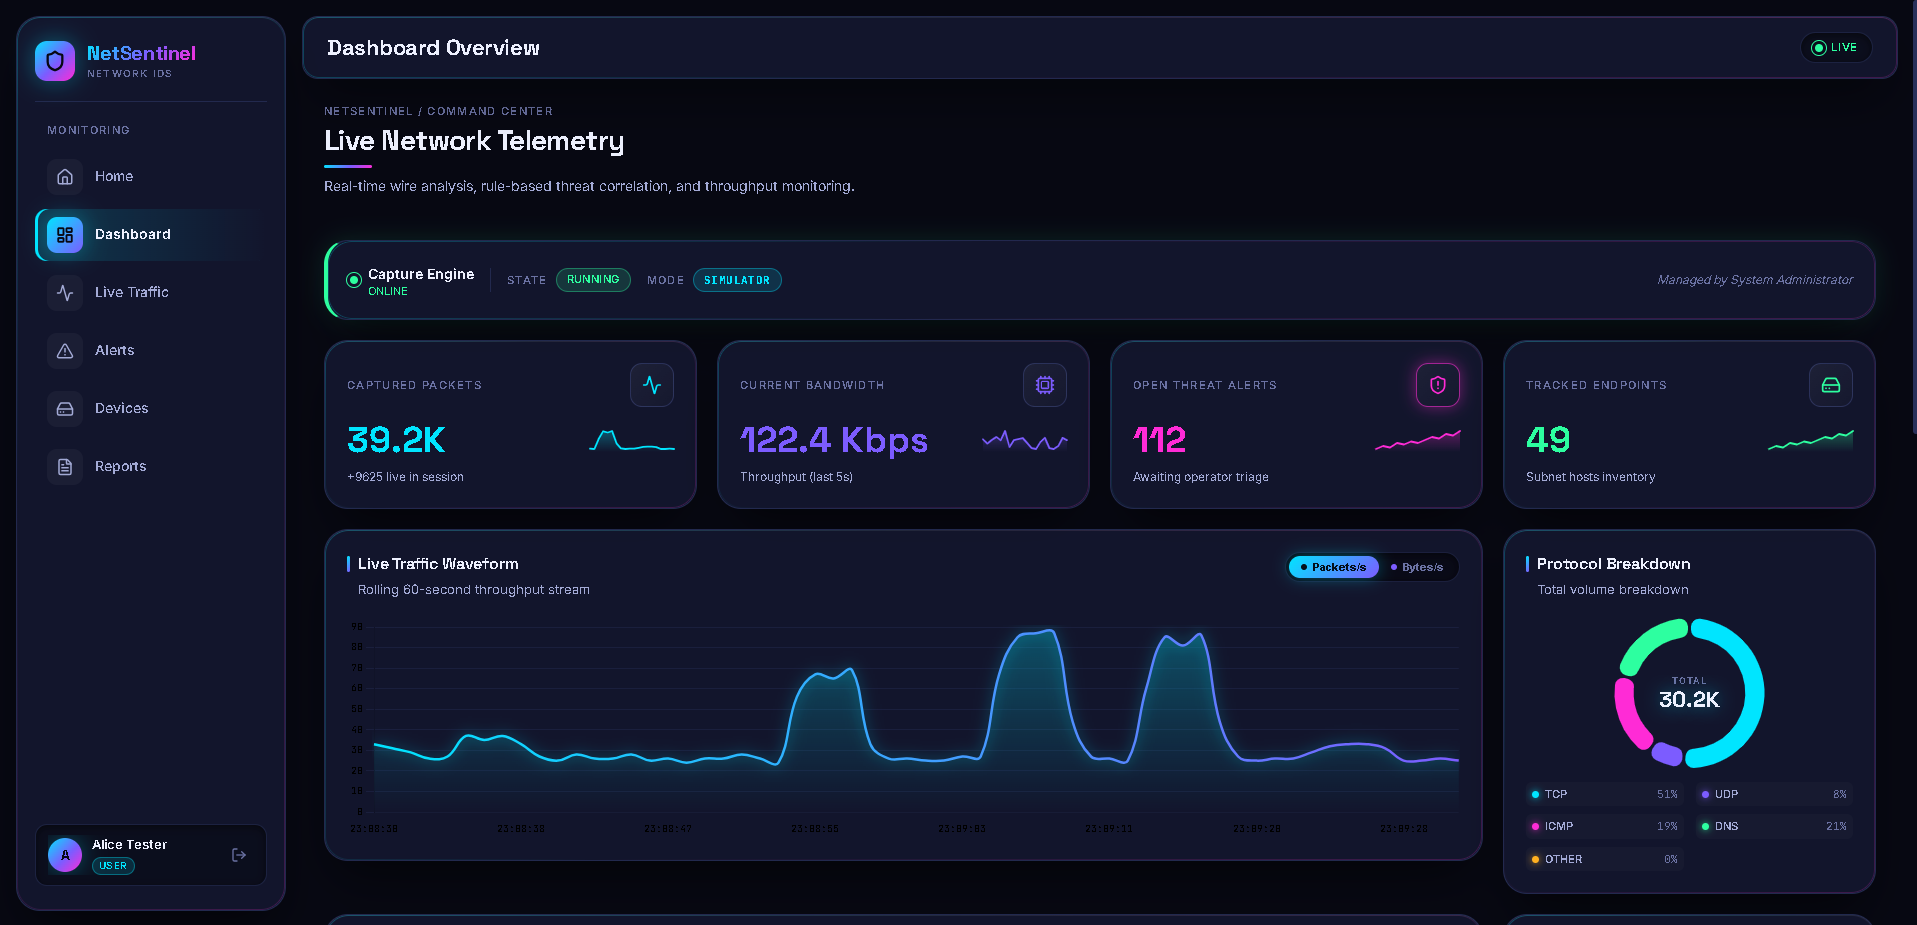
\includegraphics[width=0.88\linewidth,height=0.38\textheight,keepaspectratio]{Screenshots/Screenshot-user-dashboard.png}
		\caption{Standard User Dashboard with Real-Time Telemetry}
		\label{fig:screen-user-dash}
	\end{figure}
	
	\par
	Figure~\ref{fig:screen-admin-dash} shows the Administrator Operations Dashboard, which incorporates the privileged Capture Control Bar enabling real-time switching between Simulator and Live interface capture modes.
	
	\begin{figure}[H]
		\centering
		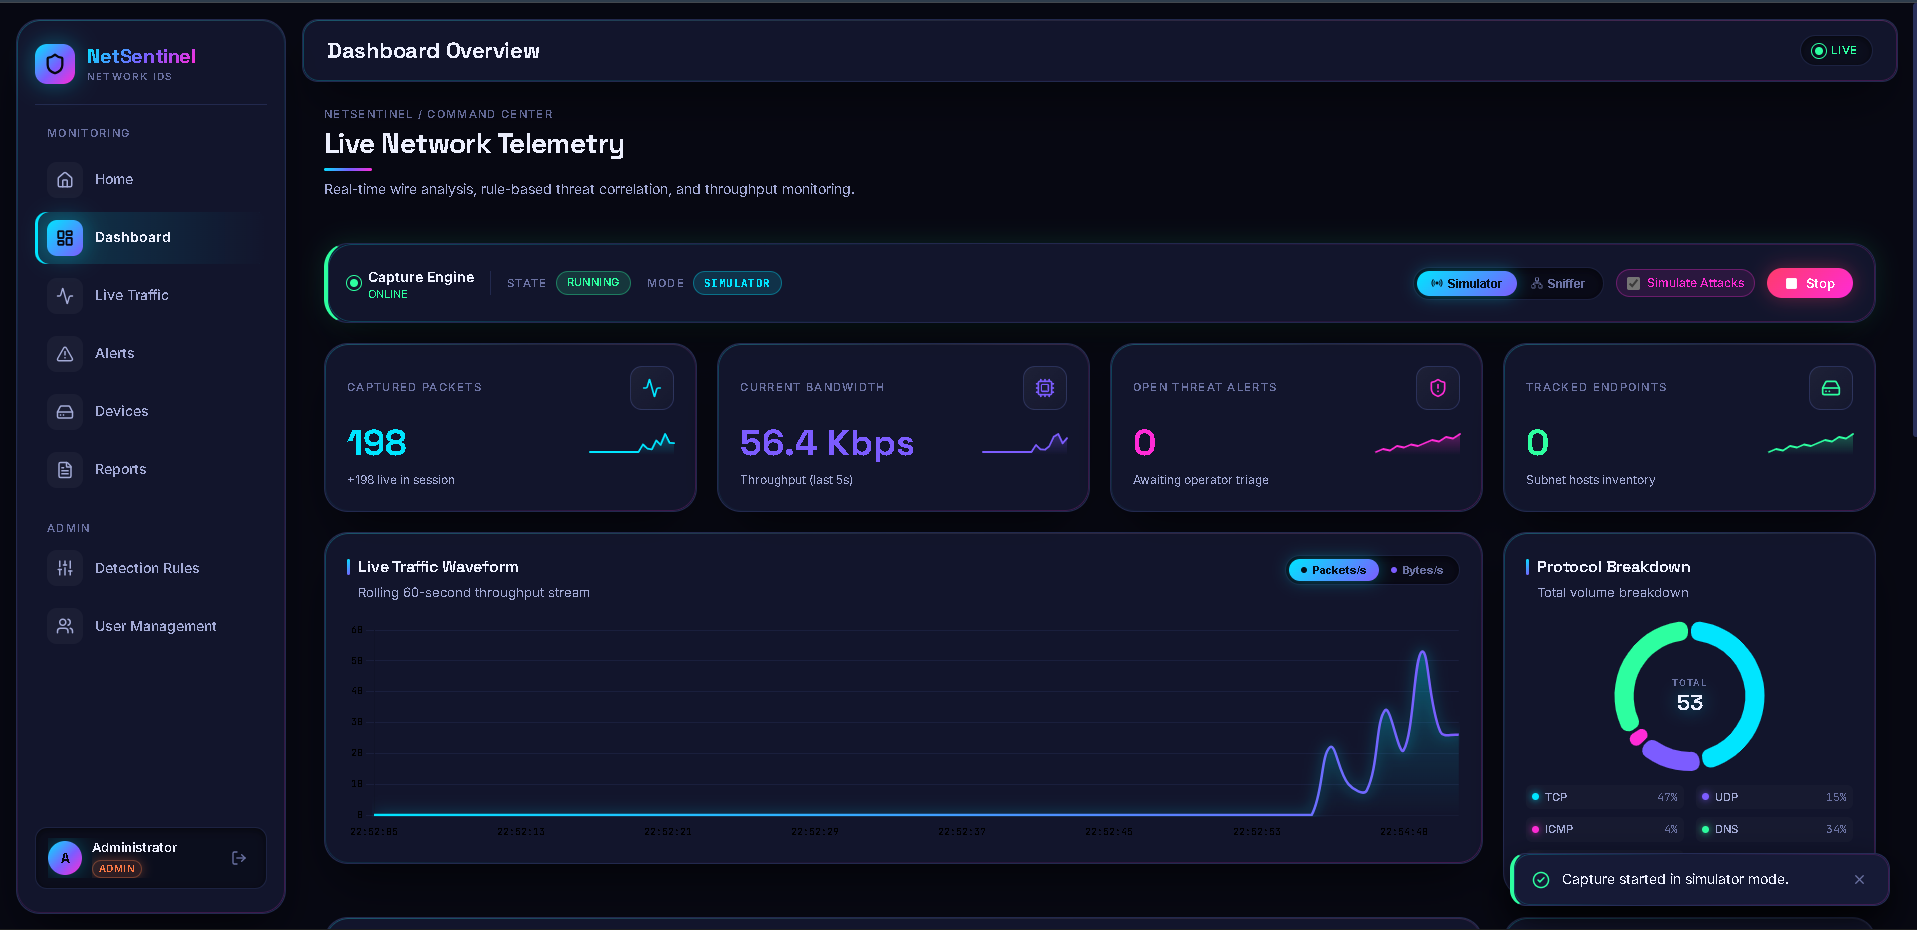
\includegraphics[width=0.88\linewidth,height=0.38\textheight,keepaspectratio]{Screenshots/Screenshot-admin-dashboard.png}
		\caption{Administrator Operations Dashboard with Capture Controls}
		\label{fig:screen-admin-dash}
	\end{figure}
	
	\clearpage
	\par
	Figure~\ref{fig:screen-traffic} shows the Live Traffic Explorer interface, displaying captured packet frames in a searchable, paginated table with protocol filtering controls.
	
	\begin{figure}[H]
		\centering
		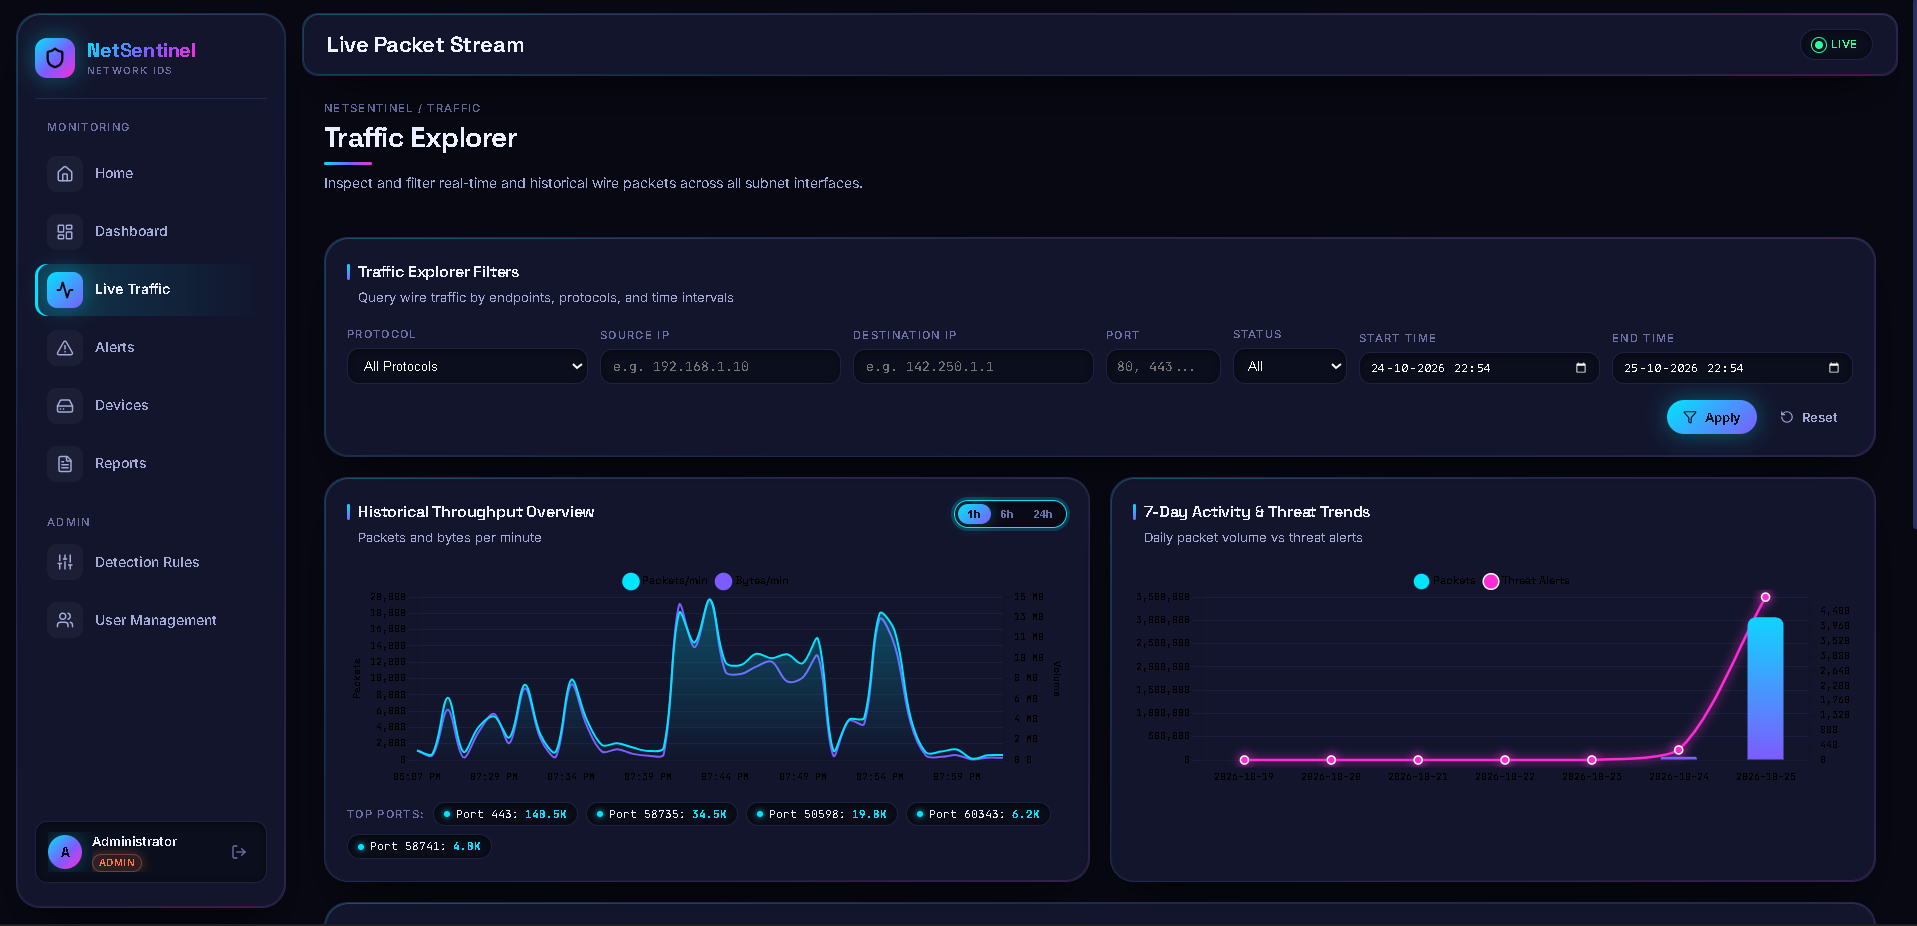
\includegraphics[width=0.88\linewidth,height=0.38\textheight,keepaspectratio]{Screenshots/Screenshot-admin-live-traffic.png}
		\caption{Live Traffic Explorer with Protocol Filters}
		\label{fig:screen-traffic}
	\end{figure}
	
	\par
	Figure~\ref{fig:screen-investigation} shows the Threat Investigation Drawer, which slides out to present parsed packet headers, rule trigger descriptions, and raw hexadecimal payload dumps.
	
	\begin{figure}[H]
		\centering
		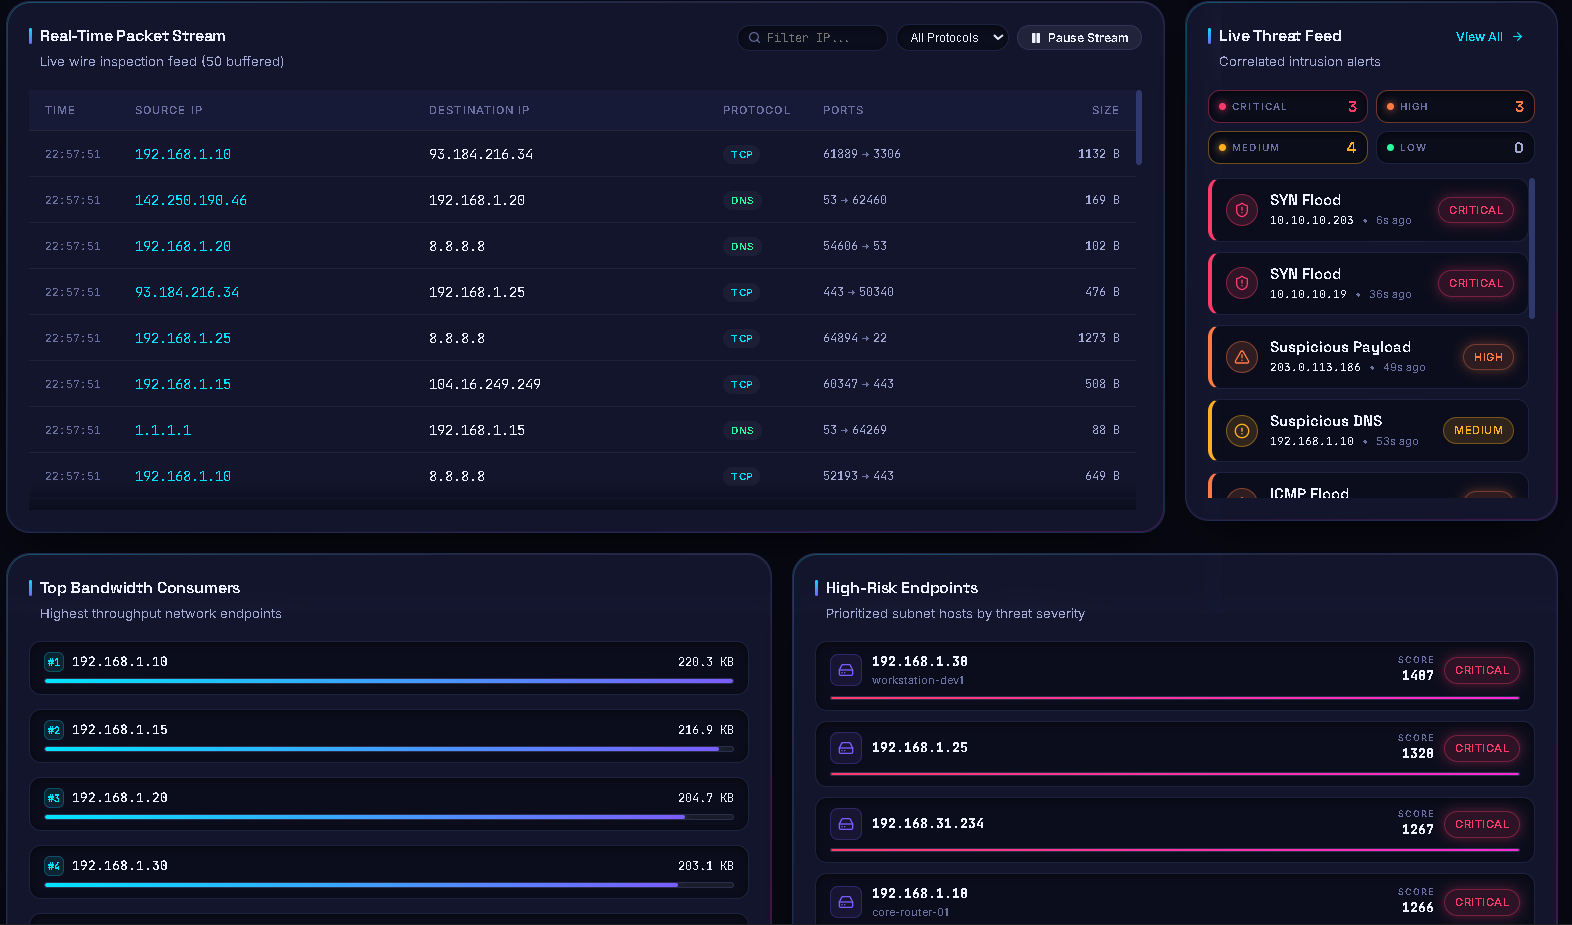
\includegraphics[width=0.88\linewidth,height=0.38\textheight,keepaspectratio]{Screenshots/Screenshot-admin-realtime-anyalysing.png}
		\caption{Incident Investigation Drawer with Hex Payload Preview}
		\label{fig:screen-investigation}
	\end{figure}
	
	\clearpage
	\par
	Figure~\ref{fig:screen-alerts} illustrates the Security Alerts Management interface, displaying categorized security incidents, severity badges, and administrative triage action buttons.
	
	\begin{figure}[H]
		\centering
		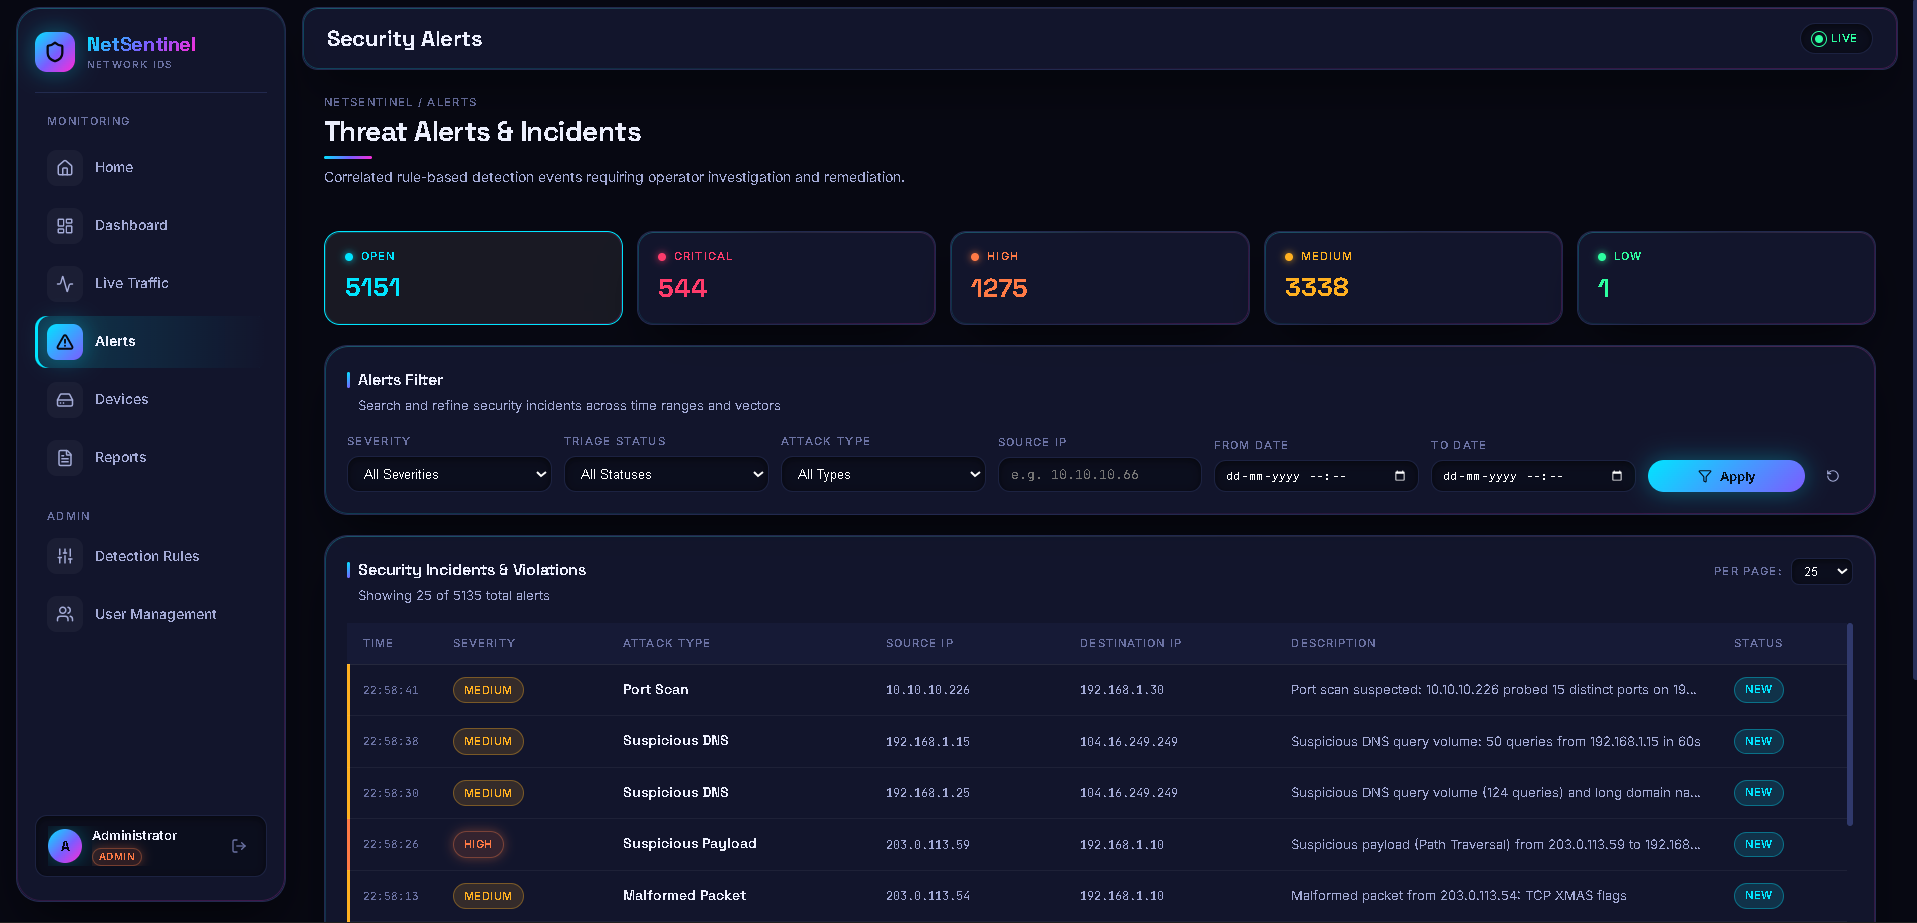
\includegraphics[width=0.86\linewidth,height=0.19\textheight,keepaspectratio]{Screenshots/Screenshot-admin-alerts.png}
		\caption{Security Alerts Management and Triage View}
		\label{fig:screen-alerts}
	\end{figure}
	
	\par
	Figure~\ref{fig:screen-devices} displays the Discovered Network Devices inventory, showing active subnet hosts categorized by device type along with their empirical behavioral risk scores.
	
	\begin{figure}[H]
		\centering
		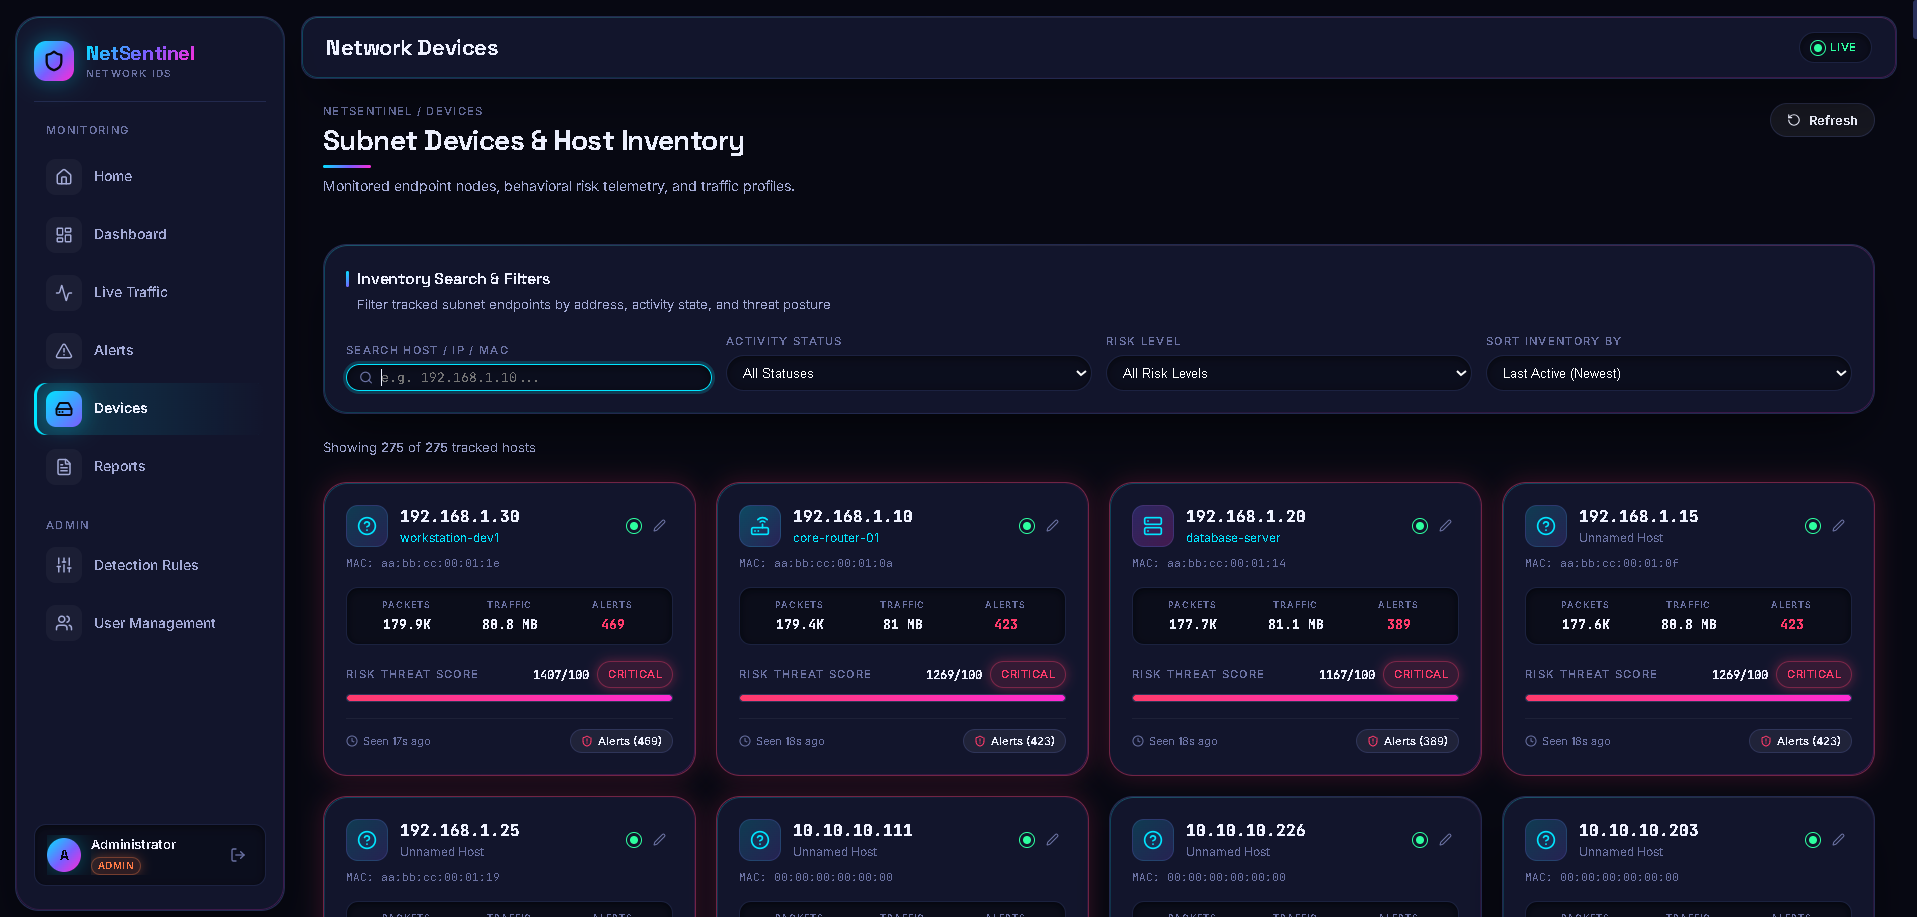
\includegraphics[width=0.86\linewidth,height=0.19\textheight,keepaspectratio]{Screenshots/Screenshot-admin-tracked-devices.png}
		\caption{Discovered Network Devices Inventory with Risk Scores}
		\label{fig:screen-devices}
	\end{figure}
	

	\par
	Figure~\ref{fig:screen-rules} shows the Detection Rules Management interface, enabling administrators to tune heuristic thresholds, adjust time windows, and toggle rules between active and disabled states.
	
	\begin{figure}[H]
		\centering
		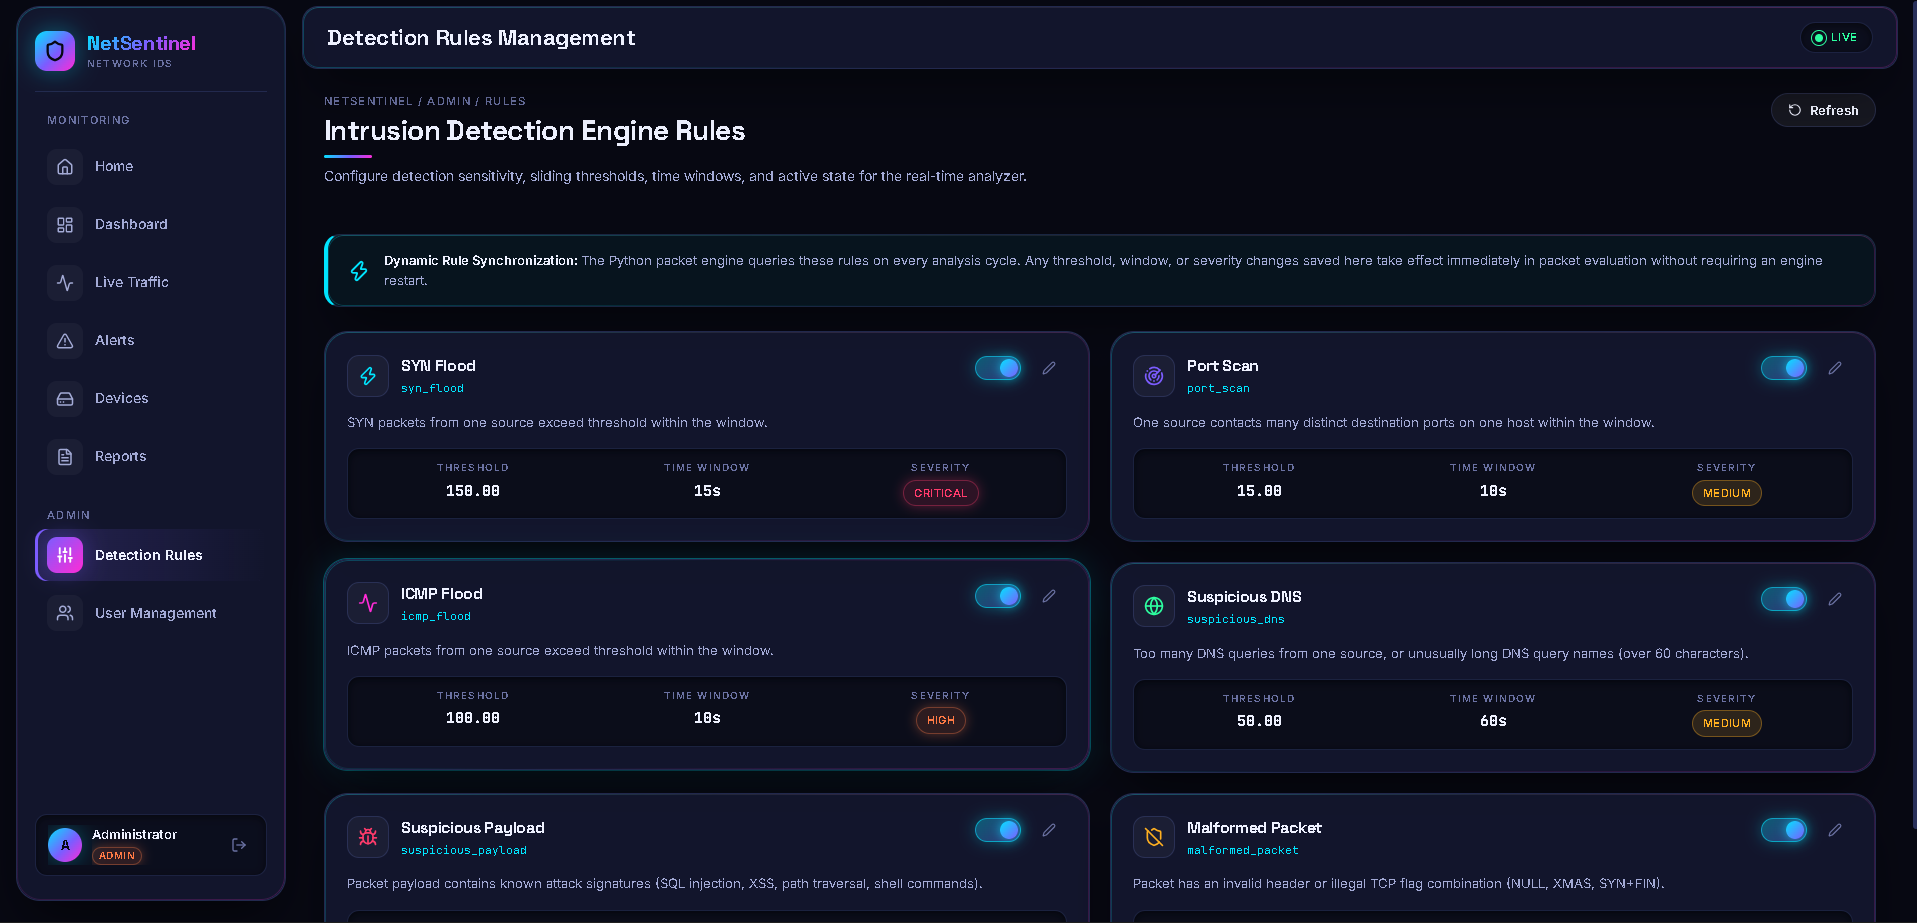
\includegraphics[width=0.86\linewidth,height=0.19\textheight,keepaspectratio]{Screenshots/Screenshot-admin-detection-rules.png}
		\caption{Detection Rules Configuration and Sensitivity Tuning}
		\label{fig:screen-rules}
	\end{figure}
	
	% =====================================================================
	%  CHAPTER 8
	% =====================================================================
	\chapter{CONCLUSION AND FUTURE SCOPE}
	
	\section{Conclusion}
	\par
	The design, implementation, and empirical verification of NetSentinel demonstrate that an effective, accessible, and comprehensive Network Traffic Analyzer and Intrusion Detection System can be successfully realized through a decoupled modern web architecture. By combining a high-performance Python packet capture service utilizing Scapy with an enterprise Node.js Express API and an interactive React web dashboard, the platform resolves long-standing usability and operational bottlenecks that have characterized conventional command-line and monolithic security software. The inclusion of dual operational modes—supporting both live promiscuous hardware packet sniffing via Npcap and an integrated multi-host synthetic simulator—ensures that the system can be deployed and evaluated seamlessly in both operational production environments and resource-constrained academic laboratories.
	
	NetSentinel's multi-rule sliding-window detection algorithms deliver transparent, explainable threat identification across six major cyber attack classes, ensuring security analysts are immediately informed of the exact threshold parameters, protocol attributes, and payload signatures responsible for triggering each security incident. The integration of bidirectional WebSocket communication guarantees low-latency telemetry streaming, while the normalized MySQL database schema preserves audit-compliant event histories and facilitates the on-demand generation of executive PDF summaries and raw CSV forensic extracts. The project successfully fulfills all stated objectives, establishing a reliable, extensible, and user-centric foundation for localized network observability, threat triage, and cybersecurity education.
	
	\section{Future Scope}
	\begin{enumerate}
		\item \textbf{Machine Learning Anomaly Classification:}
		Integrating unsupervised anomaly detection algorithms (such as Isolation Forests or lightweight Autoencoders) alongside the heuristic rules to detect subtle, low-frequency zero-day attacks that do not trigger hard volumetric thresholds.
		
		\item \textbf{Automated Active Defense and Firewall Integration:}
		Expanding the platform into an Intrusion Prevention System (IPS) capable of automatically executing host firewall rules (such as Windows Defender Firewall or Linux iptables) to isolate and drop malicious source IP connections upon threshold breach.
		
		\item \textbf{Encrypted Traffic Analysis via TLS Fingerprinting:}
		Implementing JA3 and JA4 TLS fingerprinting mechanisms to classify encrypted malicious command-and-control communication channels without requiring full payload decryption.
		
		\item \textbf{Automated Email and SMS Incident Notification Hooks:}
		Integrating automated alerting channels such as SMTP email alerts, Webhook notifications, and SMS triggers to dispatch immediate incident alerts to security personnel when Critical threats are detected.
		
		\item \textbf{Distributed Multi-Probe Sensor Architecture:}
		Extending the Python capture service into a distributed remote sensor agent capable of capturing telemetry across multiple remote subnet gateways and forwarding aggregated streams to a centralized cloud-hosted NetSentinel server.
		
		\item \textbf{Deep PCAP File Ingestion and Playback Engine:}
		Providing an administrative upload interface that allows security analysts to upload historical .pcap capture files directly through the web portal for retroactive offline threat analysis and playback.
	\end{enumerate}
	
	\vspace{1.5cm}
	
	% =====================================================================
	%  REFERENCES
	% =====================================================================
	\renewcommand{\bibname}{\uppercase{REFERENCES}}
	
	\begin{thebibliography}{999}
		
		\addcontentsline{toc}{chapter}{\hspace{0.19in} REFERENCES}
		
		\bibitem{one}
		A. Tamrakar, J. Chaturvedi, M. Poddar, and S. Kumari, Network Traffic Analyzer: Real-Time Detection and Malicious Activity Identification,'' \textit{International Journal on Advanced Computer Theory and Engineering}, vol. 15, no. 1, pp. 45--52, 2026.
		
		\bibitem{two}
		{\L}. Wawrowski, A. Bia{\l}as, A. Kajzer, A. Koz{\l}owski, R. Kurianowicz, M. Sikora, A. Szyma{\'n}ska-Kwiecie{\'n}, M. Uchro{\'n}ski, M. Bia{\l}czak, M. Olejnik, and M. Michalak, Anomaly Detection Module for Network Traffic Monitoring in Public Institutions,'' \textit{Sensors}, vol. 23, no. 6, Art. no. 2974, 2023. DOI: 10.3390/s23062974.
		
		\bibitem{three}
		D. Oroian, R. Bolboaca, A.-S. Roman, and V. Dobrota, Network Intrusion Detection System Using Anomaly Detection Techniques,'' in \textit{Proc. IEEE 20th International Conference on Intelligent Computer Communication and Processing (ICCP)}, Cluj-Napoca, Romania, 2024, pp. 93--100. DOI: 10.1109/ICCP63038.2024.10777174.
		
		\bibitem{four}
		J. Buzzio-Garc{\'i}a, J. Vergara, S. R{\'i}os-Guiral, C. Garz{\'o}n, S. Guti{\'e}rrez, J. F. Botero, J. L. Quiroz-Arroyo, and J. A. P{\'e}rez-D{\'i}az, Exploring Traffic Patterns Through Network Programmability: Introducing SDNFlow, a Comprehensive OpenFlow-Based Statistics Dataset for Attack Detection,'' \textit{IEEE Access}, vol. 12, pp. 42163--42180, 2024. DOI: 10.1109/ACCESS.2024.3377759.
		
		\bibitem{five}
		S. Racherla, et al., Deep-IDS: A Real-Time Intrusion Detector for IoT Nodes Using Deep Learning,'' \textit{IEEE Access}, vol. 12, pp. 62140--62155, 2024. DOI: 10.1109/ACCESS.2024.3396461.
		
		\bibitem{six}
		NetSentinel Project Repository, Available: https://github.com/sameersha/netsentinel, Accessed: Oct. 2026.
		
	\end{thebibliography}
	
\end{document}
